%%%%%%%%%%%%%%%%%%%%%%%%%%%%%%%%%%%%%%%%%
% Classicthesis Typographic Thesis
% LaTeX Template
% Version 1.4 (1/1/16)
%
% This template has been downloaded from:
% http://www.LaTeXTemplates.com
%
% Original author:
% 
% License:
% GNU General Public License (v2)
%
% General Tips:
% 1) Make sure to edit the classicthesis-config.file
% 2) New enumeration (A., B., C., etc in small caps): \begin{aenumerate} \end{aenumerate}
% 3) For margin notes: \marginpar or \graffito{}
% 4) Do not use bold fonts in this style, it is designed around them
% 5) Use tables as in the examples
% 6) See classicthesis-preamble.sty for useful commands
%
%%%%%%%%%%%%%%%%%%%%%%%%%%%%%%%%%%%%%%%%%

%----------------------------------------------------------------------------------------
%	PACKAGES AND OTHER DOCUMENT CONFIGURATIONS
%----------------------------------------------------------------------------------------

\documentclass[
		%headinclude=true,
		%twoside,
		openright,
		titlepage,
		numbers=noenddot,
		headinclude,
		%1headlines,
	 	%footinclude=true,
	 	cleardoublepage=empty,
		dottedtoc, % Make page numbers in the table of contents flushed right with dots leading to them
		%BCOR=5mm,
		paper=a4,
		fontsize=12pt, % Binding correction, paper type and font size
		french,
		american, % Languages, change this to your language(s)
		]{scrreprt} 
                
% Includes the file which contains all the document configurations and packages - make sure to edit this file
%%%%%%%%%%%%%%%%%%%%%%%%%%%%%%%%%%%%%%%%%
% Classicthesis Typographic Thesis
% Configuration File
%
% This file has been downloaded from:
% http://www.LaTeXTemplates.com
%
% Original author:
% André Miede (http://www.miede.de) with extensive commenting changes by:
% Vel (vel@LaTeXTemplates.com)
%
% License:
% GNU General Public License (v2)
%
% Important note:
% The main lines to change in this file are in the DOCUMENT VARIABLES
% section, the rest of the file is for advanced configuration.
%
%%%%%%%%%%%%%%%%%%%%%%%%%%%%%%%%%%%%%%%%%

%----------------------------------------------------------------------------------------
%	CHARACTER ENCODING
%----------------------------------------------------------------------------------------

\PassOptionsToPackage{utf8}{inputenc} % Set the encoding of your files. UTF-8 is the only sensible encoding nowadays. If you can't read äöüßáéçèê∂åëæƒÏ€ then change the encoding setting in your editor, not the line below. If your editor does not support utf8 use another editor!
\usepackage{inputenc}

%----------------------------------------------------------------------------------------
%	DOCUMENT VARIABLES
%	Fill in the lines below to enter your information into the thesis template
%	Each of the commands can be cited anywhere in the thesis
%----------------------------------------------------------------------------------------

% Remove drafting to get rid of the '[ Date - classicthesis version 4.0 ]' text at the bottom of every page
\PassOptionsToPackage{eulerchapternumbers,listings,drafting, pdfspacing, subfig,beramono,eulermath,parts}{classicthesis}
% Available options: drafting parts nochapters linedheaders eulerchapternumbers beramono eulermath pdfspacing minionprospacing tocaligned dottedtoc manychapters listings floatperchapter subfig

%\newcommand{\myTitle}{Apprentissage supervisé, la reconnaissance des plaques d'immatriculation utilisant l'algorithme de descente de gradient stochastique\xspace}
\newcommand{\myTitle}{Machine Learning: Étude de la minimisation d'erreur dans l'apprentissage supervisé, avec une application de la technologie ANPR\xspace}
\newcommand{\myTitleEn}{Supervised learning, License Recognition using the stochastic gradient descent algorithm\xspace}
\newcommand{\mySubtitle}{TFC\xspace}
\newcommand{\myDegree}{Licencié en informatique\xspace}
\newcommand{\myName}{\textsc{TSHELEKA KAJILA} Hassan\xspace}
%\newcommand{\myProf}{Prof. BAGULA Antoine\xspace}
\newcommand{\myProf}{Prof. MASAKUNA Jordan\xspace}
\newcommand{\myOtherProf}{Put name here\xspace}
\newcommand{\mySupervisor}{Mr. \textsc{MWAHU} Auguste\xspace}
\newcommand{\myFaculty}{Sciences Informatiques\xspace}
\newcommand{\myDepartment}{\href{https://www.unhorizons.org}{Calcul Scientifique}\xspace}
\newcommand{\myUni}{\href{http://www.unhorizons.org}{Université Nouveaux Horizons}\xspace}
\newcommand{\myLocation}{Lubumbashi\xspace}
\newcommand{\myTime}{Janvier 2022\xspace}
\newcommand{\myVersion}{version 4.2\xspace}

%----------------------------------------------------------------------------------------
%	USEFUL COMMANDS
%----------------------------------------------------------------------------------------

\newcommand{\ie}{i.\,e.}
\newcommand{\Ie}{I.\,e.}
\newcommand{\eg}{e.\,g.}
\newcommand{\Eg}{E.\,g.} 
\newcommand{\cf}{\emph{cf.}} 

\newcounter{dummy} % Necessary for correct hyperlinks (to index, bib, etc.)
\providecommand{\mLyX}{L\kern-.1667em\lower.25em\hbox{Y}\kern-.125emX\@}
\newlength{\abcd} % for ab..z string length calculation

%----------------------------------------------------------------------------------------
%	PACKAGES
%----------------------------------------------------------------------------------------

\usepackage{lipsum} % Used for inserting dummy 'Lorem ipsum' text into the template

%------------------------------------------------

%\PassOptionsToPackage{ngerman,american}{babel}  % Change this to your language(s)
% Spanish languages need extra options in order to work with this template
%\PassOptionsToPackage{spanish,es-lcroman}{babel}
\usepackage{babel}

%------------------------------------------------			

\usepackage{csquotes}
\PassOptionsToPackage{%
%backend=biber, % Instead of bibtex
backend=bibtex8,bibencoding=ascii,%
language=auto,%
style=numeric-comp,%
%style=authoryear-comp, % Author 1999, 2010
%bibstyle=authoryear,dashed=false, % dashed: substitute rep. author with ---
sorting=nyt, % name, year, title
maxbibnames=10, % default: 3, et al.
%backref=true,%
natbib=true % natbib compatibility mode (\citep and \citet still work)
}{biblatex}
\usepackage{biblatex}
 
 %------------------------------------------------

\PassOptionsToPackage{fleqn}{amsmath} % Math environments and more by the AMS 
 \usepackage{amsmath}
 
 %------------------------------------------------

\PassOptionsToPackage{T1}{fontenc} % T2A for cyrillics
\usepackage{fontenc}

%------------------------------------------------

\usepackage{textcomp} % Fix warning with missing font shapes

%------------------------------------------------

\usepackage{scrhack} % Fix warnings when using KOMA with listings package  

%------------------------------------------------

\usepackage{xspace} % To get the spacing after macros right

%------------------------------------------------

\usepackage{mparhack} % To get marginpar right

%------------------------------------------------

\usepackage{fixltx2e} % Fixes some LaTeX stuff 

%------------------------------------------------

\PassOptionsToPackage{smaller}{acronym} % Include printonlyused in the first bracket to only show acronyms used in the text
\usepackage{acronym} % Nice macros for handling all acronyms in the thesis

%\renewcommand*{\acsfont}[1]{\textssc{#1}} % For MinionPro
\renewcommand*{\aclabelfont}[1]{\acsfont{#1}}

%------------------------------------------------

\PassOptionsToPackage{pdftex}{graphicx}
\usepackage{graphicx} 

%----------------------------------------------------------------------------------------
%	FLOATS: TABLES, FIGURES AND CAPTIONS SETUP
%----------------------------------------------------------------------------------------

\usepackage{tabularx} % Better tables
\setlength{\extrarowheight}{3pt} % Increase table row height
\newcommand{\tableheadline}[1]{\multicolumn{1}{c}{\spacedlowsmallcaps{#1}}}
\newcommand{\myfloatalign}{\centering} % To be used with each float for alignment
\usepackage{caption}
\captionsetup{font=small}
\usepackage{subfig}  

%----------------------------------------------------------------------------------------
%	CODE LISTINGS SETUP
%----------------------------------------------------------------------------------------

\usepackage{listings} 
%\lstset{emph={trueIndex,root},emphstyle=\color{BlueViolet}}%\underbar} % For special keywords
\lstset{language=[LaTeX]Tex,%C++ % Specify the language(s) for listings here
	morekeywords={PassOptionsToPackage,selectlanguage},
	keywordstyle=\color{RoyalBlue}, % Add \bfseries for bold
	basicstyle=\small\ttfamily, % Makes listings a smaller font size and a different font
	%identifierstyle=\color{NavyBlue}, % Color of text inside brackets
	commentstyle=\color{Green}\ttfamily, % Color of comments
	stringstyle=\rmfamily, % Font type to use for strings
	numbers=left, % Change left to none to remove line numbers
	numberstyle=\scriptsize, % Font size of the line numbers
	stepnumber=5, % Increment of line numbers
	numbersep=8pt, % Distance of line numbers from code listing
	showstringspaces=false, % Sets whether spaces in strings should appear underlined
	breaklines=true, % Force the code to stay in the confines of the listing box
	%frameround=ftff, % Uncomment for rounded frame
	%frame=single, % Frame border - none/leftline/topline/bottomline/lines/single/shadowbox/L
	belowcaptionskip=.75\baselineskip % Space after the "Listing #: Desciption" text and the listing box
}

%----------------------------------------------------------------------------------------
%	HYPERREFERENCES
%----------------------------------------------------------------------------------------

\PassOptionsToPackage{pdftex,hyperfootnotes=false,pdfpagelabels}{hyperref}
\usepackage{hyperref}  % backref linktocpage pagebackref
\pdfcompresslevel=9
\pdfadjustspacing=1

\hypersetup{
	% Uncomment the line below to remove all links (to references, figures, tables, etc), useful for b/w printouts
	%draft, 
	colorlinks=true, linktocpage=true, pdfstartpage=3, pdfstartview=FitV,
	% Uncomment the line below if you want to have black links (e.g. for printing black and white)
	%colorlinks=false, linktocpage=false, pdfborder={0 0 0}, pdfstartpage=3, pdfstartview=FitV, 
	breaklinks=true, pdfpagemode=UseNone, pageanchor=true, pdfpagemode=UseOutlines,%
	plainpages=false, bookmarksnumbered, bookmarksopen=true, bookmarksopenlevel=1,%
	hypertexnames=true, pdfhighlight=/O,%nesting=true,%frenchlinks,%
	urlcolor=webbrown, linkcolor=RoyalBlue, citecolor=webgreen, %pagecolor=RoyalBlue,%
	    %urlcolor=Black, linkcolor=Black, citecolor=Black, %pagecolor=Black,%
	%------------------------------------------------
	% PDF file meta-information
	pdftitle={\myTitle},
	pdfauthor={\textcopyright\ \myName, \myUni, \myFaculty},
	pdfsubject={thesis},
	pdfkeywords={ECW},
	pdfcreator={},
	pdfproducer={LaTeX}
	%------------------------------------------------
}

%----------------------------------------------------------------------------------------
%	AUTOREFERENCES SETUP
%	Redefines how references in text are prefaced for different 
%	languages (e.g. "Section 1.2" or "section 1.2")
%----------------------------------------------------------------------------------------

\makeatletter
\@ifpackageloaded{babel}
{
\addto\extrasamerican{
\renewcommand*{\figureautorefname}{Figure}
\renewcommand*{\tableautorefname}{Table}
\renewcommand*{\partautorefname}{Part}
\renewcommand*{\chapterautorefname}{Chapter}
\renewcommand*{\sectionautorefname}{Section}
\renewcommand*{\subsectionautorefname}{Section}
\renewcommand*{\subsubsectionautorefname}{Section}
}
\addto\extrasngerman{
\renewcommand*{\paragraphautorefname}{Absatz}
\renewcommand*{\subparagraphautorefname}{Unterabsatz}
\renewcommand*{\footnoteautorefname}{Fu\"snote}
\renewcommand*{\FancyVerbLineautorefname}{Zeile}
\renewcommand*{\theoremautorefname}{Theorem}
\renewcommand*{\appendixautorefname}{Anhang}
\renewcommand*{\equationautorefname}{Gleichung}
\renewcommand*{\itemautorefname}{Punkt}
}
\providecommand{\subfigureautorefname}{\figureautorefname} % Fix to getting autorefs for subfigures right
}{\relax}
\makeatother

%----------------------------------------------------------------------------------------

\usepackage{classicthesis} 

%----------------------------------------------------------------------------------------
%	CHANGING TEXT AREA 
%----------------------------------------------------------------------------------------

%\linespread{1.05} % a bit more for Palatino
%\areaset[current]{312pt}{761pt} % 686 (factor 2.2) + 33 head + 42 head \the\footskip
%\setlength{\marginparwidth}{7em}%
%\setlength{\marginparsep}{2em}%

%----------------------------------------------------------------------------------------
%	USING DIFFERENT FONTS
%----------------------------------------------------------------------------------------

%\usepackage[oldstylenums]{kpfonts} % oldstyle notextcomp
%\usepackage[osf]{libertine}
%\usepackage[light,condensed,math]{iwona}
%\renewcommand{\sfdefault}{iwona}
%\usepackage{lmodern} % <-- no osf support :-(
%\usepackage{cfr-lm} % 
%\usepackage[urw-garamond]{mathdesign} <-- no osf support :-(
%\usepackage[default,osfigures]{opensans} % scale=0.95 
%\usepackage[sfdefault]{FiraSans}
%\usepackage{lipsum}
\usepackage{float}
\usepackage{pdfpages}
\usepackage{wrapfig}
%\usepackage{hyphsubst}

\addbibresource{bibliography/biblio.bib} % The file housing your bibliography
%\addbibresource[label=ownpubs]{Self_Publications.bib} % Uncomment for optional self-publications

%\hyphenation{Put special hyphenation here}

\areaset{15cm}{25.8cm}

\parindent 0pt
\parskip 6pt

%%%%%%%%%%%%%%%%%%%%%%%%%%%%%%%%%%%%%%%%%%%%%%%%%

\newtheorem{thm}{Theorem}
%\newcommand{\textit}{\italic}
\newcommand{\italic}[1]{\textit{#1}}
\newcommand{\n}{\\}

\begin{document}

%\renewcommand{\thesubsubsection}{\alph{subsection}}
%\renewcommand{\thesubsubsection}{\alph{subsubsection}.}
\renewcommand\thesubsubsection{\alph{subsubsection}.}
\setcounter{chapter}{-1}


\frenchspacing % Reduces space after periods to make text more compact

\raggedbottom % Makes all pages the height of the text on that page

\selectlanguage{french} % Select your default language - e.g. american or ngerman

%\renewcommand*{\bibname}{new name} % Uncomment to change the name of the bibliography
%\setbibpreamble{} % Uncomment to include a preamble to the bibliography - some text before the reference list starts

\pagenumbering{roman} % Roman page numbering prior to the start of the thesis content (i, ii, iii, etc)

\pagestyle{plain} % Suppress headers for the pre-content pages

%----------------------------------------------------------------------------------------
%	PRE-CONTENT THESIS PAGES
%----------------------------------------------------------------------------------------

% Title Page

\begin{titlepage}

%\begin{addmargin}[-1cm]{-3cm}
\begin{center}
\large

\vspace*{.03\textheight}


 

%\text{word or phrase}
%\vspace{1.5cm} 

\includegraphics[width=12cm]{images/logo_unh} \\[0.75cm]

{\LARGE{{\textsc{FACULT\'E DES SCIENCES INFORMATIQUES}}} }\\[0.2cm]

{\LARGE{{{Calcul Scientifique}}} }\\
\medskip % Picture

\vspace{2.5cm} 

%{\hrule width5cm}  % Horizontal line
\begin{center}
	\rule{0.9\textwidth}{.2pt}
\end{center}
\vspace{0.2cm}
{\LARGE \bfseries {\myTitle}}%\vspace{0.4cm} % Thesis title
%{\hrule width5cm} 
\begin{center}
	\rule{0.9\textwidth}{.2pt}
\end{center}

%\color{Maroon}\spacedallcaps{\myTitle} \\ \bigskip % Thesis title

\textit{Travail de fin d’études présenté  et défendu en vue de l’obtention du grade de licencié en \myDepartment.}\\[2cm]

\begin{minipage}[t]{0.4\textwidth}
	\begin{flushleft} \large
		%\emph{Auteur:}\\
		%{\myName} % Author name - remove the \href bracket to remove the link
	\end{flushleft}
\end{minipage}
\begin{minipage}[t]{0.5\textwidth}
	\begin{flushright} \large
		\emph{Auteur:}
		\textbf{{\myName}}\\
		\emph{Directeur:} 
		%\href{https://cs.uwc.ac.za/anttoine-bagula/}{\myProf} % Supervisor name - remove the \href bracket to remove the link
		\textbf{{\myProf}}  
	\end{flushright}
\end{minipage}\\[3cm]

%\spacedlowsmallcaps{\myName} % Your name

\vfill


% Travail de fin d’études présenté en vue de l’obtention du grade de licence en Sciences Informatiques
%Mémoire présenté à la Faculté des \myFaculty en vue de l'obtention du grade de \myDegree.
%Travail de fin d’études présenté en vue de l’obtention du grade de \myDegree en Sciences Informatiques.

 % University requirement text
%\textit{département}\\[0.2cm]
%\myDepartment \\[0.75cm]
%\medskip % Thesis subtitle
%\myDegree \\
%\myDepartment \\
%\myFaculty \\
%\myUni \\ \bigskip

{\large \today}\\

%\myTime\ - % Time and version



\end{center}
%\end{addmargin}

\end{titlepage} % Main title page
%%
\includegraphics[]{gfx/garde} 

%
\includepdf[pages={1}]{gfx/garde.pdf}

%#
%% Back of the title page

\thispagestyle{empty}

\hfill

\vfill

\noindent\myName: \textit{\myTitle,} \mySubtitle, %\myDegree, 
\textcopyright\ \myTime

% You may wish to do something with the back of the title page, such as including your supervisors, location or time frame of the work. Below is an example of doing so although you may want to tweak it to your liking.

%\bigskip

%\noindent\spacedlowsmallcaps{Supervisors}: \\
%\myProf \\
%\myOtherProf \\ 
%\mySupervisor

%\medskip \\

%\noindent\spacedlowsmallcaps{Location}: \\
%\myLocation

%\medskip \\

%\noindent\spacedlowsmallcaps{Time Frame}: \\
%\myTime
 % Back of the title page


%\cleardoublepage% Dedication

\thispagestyle{empty}
\refstepcounter{dummy}

\pdfbookmark[1]{Dedication}{Dedication} % Bookmark name visible in a PDF viewer

\vspace*{3cm}

\begin{center}
\emph{Ohana} means family. \\
Family means nobody gets left behind, or forgotten. \\ \medskip
--- Lilo \& Stitch    
\end{center}

\medskip

\begin{center}
Dedicated to the loving memory of Rudolf Miede. \\ \smallskip
1939\,--\,2005
\end{center} % Dedication page
%\cleardoublepage\include{FrontBackMatter/Foreword} % Uncomment and create a Foreword.tex to include a foreword

\cleardoublepage% Abstract

\renewcommand{\abstractname}{Résumé} % Uncomment to change the name of the abstract

\pdfbookmark[1]{Résumé}{Résumé} % Bookmark name visible in a PDF viewer
\addcontentsline{toc}{chapter}{Résumé}
\begingroup
\let\clearpage\relax
\let\cleardoublepage\relax
\let\cleardoublepage\relax

\chapter*{Résumé}
	Au cours de la dernière décennie, la taille des données a augmenté plus rapidement que la vitesse des processeurs. Dans ce contexte, faire un traitement de {reconnaissance} des formes dans des images et vidéos, les ensembles de données d'entraînement pour les problèmes de détection d'objets sont généralement très volumineux et les capacités des méthodes d'apprentissage automatique statistique sont limitées par le temps de calcul plutôt que par la taille de l'échantillon. 
	
	Le cas des problèmes d'apprentissage à grande échelle implique la complexité de calcul de l'algorithme d'optimisation sous-jacent de manière non triviale. Des algorithmes d'optimisation improbables tels que la \textbf{descente de gradient stochastique} (en anglais: \textbf{Stochastic Gradient Descent} ou SGD) montre des performances étonnantes pour les problèmes à grande échelle, lorsque l'ensemble d'apprentissage est volumineux. \\
	En particulier, les variants du SGD n'utilisent qu'un seul nouvel échantillon d'apprentissage à chaque itération, sont asymptotiquement efficaces après un seul passage sur l'ensemble d'apprentissage.	
	
	Ce travail vise à proposer une méthode  intelligente, basée sur l'intelligence artificielle, qui permet aux ordinateurs et aux systèmes informatiques de dériver des informations significatives à partir d'images numériques, de vidéos et d'autres entrées visuelles, avec un coût plus bas que possible. Dans notre contexte la reconnaissance des plaques d’immatriculation des véhicules à l'aide d’un classificateur de la famille de descente de gradient stochastique. Pour minimiser la \textbf{fonction coût} du classificateur, la SGD adopte un modèle d'optimisation convexe. De plus, pour augmenter la vitesse de convergence du classificateur, la descente de gradient stochastique, à chaque étape, elle tire un échantillon aléatoire de l'ensemble des fonctions ($f_i$), de la fonction objectif, constituant la somme.
	 
	\begin{center}
		
	%\url{https://plg.uwaterloo.ca/~migod/research/beckOOPSLA.html}
	\end{center}
	\textbf{Mots clés~:} Apprentissage supervisé, vision par ordinateur, Descente de gradient stochastique, Adaline, ALPR. 

\endgroup			

\vfill

\pagebreak



\pdfbookmark[2]{Abstract}{Abstract} % Bookmark name visible in a PDF viewer

\begingroup
\let\clearpage\relax
\let\cleardoublepage\relax
\let\cleardoublepage\relax

\chapter*{Abstract}
	Over the past decade, data size has grown faster than processor speeds. In this context, doing pattern recognition processing in real-time videos, training datasets for object detection problems are usually very large, and the capabilities of statistical machine learning methods are limited by computation time rather than sample size.
	
	The case of large scale learning problems involves the computational complexity of the underlying optimization algorithm in a nontrivial way.\\
	Improbable optimization algorithms such as \textbf{Stochastic Gradient Descent} (SGD) show amazing performance for large scale problems, when the training set is bulky.\\
	In particular, SGD variants use only one new training sample at each iteration, are asymptotically efficient after a single pass over the training set.
	
	This work aims to provide an intelligent method, based on artificial intelligence, that allows computers and computer systems to derive meaningful information from digital images, videos and other visual inputs, with a lower cost. as possible. In our context the recognition of vehicle license plates using a classifier of the family of stochastic gradient descent. To minimize the \textbf{cost function} of the classifier, the SGD adopts a convex optimization model. Moreover, to increase the speed of convergence of the classifier, the stochastic gradient descent, at each step, it draws a random sample from the set of functions ($f_i$), of the objective function, constituting the sum.
	
	\begin{center}
		
		%\url{https://plg.uwaterloo.ca/~migod/research/beckOOPSLA.html}
	\end{center}
	\textbf{Key words~:} Supervised learning, computer vision, Stochastic gradient descent, Adaline, ALPR.

	

\endgroup			

\vfill % Abstract page

%\cleardoublepage% Publications - a page listing research articles written using content in the thesis

\pdfbookmark[1]{Publications}{Publications} % Bookmark name visible in a PDF viewer

\chapter*{Publications} % Publications page text

Some ideas and figures have appeared previously in the following publications:\\

\noindent Put your publications from the thesis here. The packages \texttt{multibib} or \texttt{bibtopic} etc. can be used to handle multiple different bibliographies in your document.

%\begin{refsection}[ownpubs]
%    \small
%    \nocite{*} % is local to to the enclosing refsection
%    \printbibliography[heading=none]
%\end{refsection}

%\emph{Attention}: This requires a separate run of \texttt{bibtex} for your \texttt{refsection}, \eg, \texttt{ClassicThesis1-blx} for this file. You might also use \texttt{biber} as the backend for \texttt{biblatex}. See also \url{http://tex.stackexchange.com/questions/128196/problem-with-refsection}. % Publications from the thesis page


%#
%\cleardoublepage% Acknowledgements

\pdfbookmark[1]{Acknowledgements}{Acknowledgements} % Bookmark name visible in a PDF viewer

\begin{flushright}{\slshape    
We have seen that computer programming is an art, \\ 
because it applies accumulated knowledge to the world, \\ 
because it requires skill and ingenuity, and especially \\
because it produces objects of beauty.} \\ \medskip
--- \defcitealias{knuth:1974}{Donald E. Knuth}\citetalias{knuth:1974} \citep{knuth:1974}
\end{flushright}



\bigskip

%----------------------------------------------------------------------------------------

\begingroup

\let\clearpage\relax
\let\cleardoublepage\relax
\let\cleardoublepage\relax
%\addchaptertocentry{Remerciements} 
\addcontentsline{toc}{chapter}{Remerciements}
\chapter*{Remerciements}

Arrivant à l’aboutissement de ma tâche, je me trouve dans l’obligation respectueuse de devoir présenter mes chaleureux remerciements et témoignage de ma gratitude à tous ceux qui ont contribué aimablement et avec patience à l’élaboration de ce mémoire.

Tout d’abord, je tiens à remercier profondément les membres du jury qui m’ont fait l’honneur de juger mon travail. Merci à...

Je tiens à remercier toutes les personnes qui ont contribué au succès de ... et qui m'ont aidé lors de la rédaction de ce memoire. à ceux qui m’ont beaucoup appris au cours de la redaction, et même à ceux qui ont eu la gentillesse de faire de ce ... un moment très profitable.\\

Enfin, je tiens à remercier toutes les personnes qui m'ont conseillé et relu lors de la rédaction de ce rapport de stage : ma famille, mes ami(e)s et camarade de promotion.

\endgroup % Acknowledgements page

\pagestyle{scrheadings} % Show chapter titles as headings

\cleardoublepage% Table of Contents - List of Tables/Figures/Listings and Acronyms

\refstepcounter{dummy}

\pdfbookmark[1]{\contentsname}{tableofcontents} % Bookmark name visible in a PDF viewer

\setcounter{tocdepth}{2} % Depth of sections to include in the table of contents - currently up to subsections

\setcounter{secnumdepth}{3} % Depth of sections to number in the text itself - currently up to subsubsections

\manualmark
\markboth{\spacedlowsmallcaps{\contentsname}}{\spacedlowsmallcaps{\contentsname}}
\tableofcontents 
\automark[section]{chapter}
\renewcommand{\chaptermark}[1]{\markboth{\spacedlowsmallcaps{#1}}{\spacedlowsmallcaps{#1}}}
\renewcommand{\sectionmark}[1]{\markright{\thesection\enspace\spacedlowsmallcaps{#1}}}

\clearpage

\begingroup 
\let\clearpage\relax
\let\cleardoublepage\relax
\let\cleardoublepage\relax

%----------------------------------------------------------------------------------------
%	List of Figures
%----------------------------------------------------------------------------------------

\refstepcounter{dummy}
%\addcontentsline{toc}{chapter}{\listfigurename} % Uncomment if you would like the list of figures to appear in the table of contents
\pdfbookmark[1]{\listfigurename}{lof} % Bookmark name visible in a PDF viewer


%#
\listoffigures


\vspace{8ex}
\newpage

%----------------------------------------------------------------------------------------
%	List of Tables
%----------------------------------------------------------------------------------------

%\refstepcounter{dummy}
%\addcontentsline{toc}{chapter}{\listtablename} % Uncomment if you would like the list of tables to appear in the table of contents
%\pdfbookmark[1]{\listtablename}{lot} % Bookmark name visible in a PDF viewer

%\listoftables
        
%\vspace{8ex}
%\newpage
    
%----------------------------------------------------------------------------------------
%	List of Listings
%---------------------------------------------------------------------------------------- 

%\refstepcounter{dummy}
%\addcontentsline{toc}{chapter}{\lstlistlistingname} % Uncomment if you would like the list of listings to appear in the table of contents
%\pdfbookmark[1]{\lstlistlistingname}{lol} % Bookmark name visible in a PDF viewer

%\lstlistoflistings 

%\vspace{8ex}
%\newpage
       
%----------------------------------------------------------------------------------------
%	Acronyms
%----------------------------------------------------------------------------------------

\refstepcounter{dummy}
%\addcontentsline{toc}{chapter}{Acronyms} % Uncomment if you would like the acronyms to appear in the table of contents
\pdfbookmark[1]{Acronyms}{acronyms} % Bookmark name visible in a PDF viewer

\markboth{\spacedlowsmallcaps{Acronyms}}{\spacedlowsmallcaps{Acronyms}}

\chapter*{Liste des acronymes}

\begin{acronym}[UML]
	\acro{ML}{Machine Learning}
	\acro{CV}{Computer Vision}
	
	\acro{OCR}{Optical character recognition}
	\acro{ANPR}{Automatic number-plate recognition}
	\acro{ALPR}{Automatic license plate recognition}
	
	\acro{GD}{Gradient Descent}
	\acro{SGD}{Stochastic Gradient Descent}
	\acro{ADALINE}{ADAptative LInear NEuron }
	
	
	\acro{API}{Application Programming Interface}
	\acro{UML}{Unified Modeling Language}
\end{acronym} 
                   
\endgroup


%----------------------------------------------------------------------------------------
%	Symbol
%----------------------------------------------------------------------------------------
\refstepcounter{dummy}
%\addcontentsline{toc}{chapter}{Acronyms} % Uncomment if you would like the acronyms to appear in the table of contents
\pdfbookmark[1]{Notions}{notions} % Bookmark name visible in a PDF viewer

\markboth{\spacedlowsmallcaps{Notions}}{\spacedlowsmallcaps{Notions}}

\chapter*{Notions}

\begin{tabular}{ll}
	$\mathbb{N} $ & Ensemble des entiers naturels\\
	%$\mathbb{R} $ &  \\
	$\mathbb{R}^n $ & Ensemble des réels ou  Espace euclidien de dimension $n$ \\
	$\mathbb{B}^n = \{0,1\}^n $ & Espace booléen de dimension $n$\\
	$\mathcal{O}(\cdot) $ ou $ {\Omega}(\cdot) $ & L'ordre de grandeur maximal de complexité d'un algorithme \\
	%$\mathcal{O}(\cdot) $ & Le grand O de la notation de Landeau \\
	
	
	$x = \begin{pmatrix}
		x_1 \\ \vdots \\ x_n 
	\end{pmatrix} $ & Un vecteur\\ 
	$x =  (x_1, \vdots,  x_n)^T$ & Un vecteur \\ 
	$x^T =  (x_1, \vdots,  x_n)^T$ & Un vecteur transposé \\ 
	$ \langle xy\rangle = x^Ty$  & Le produit vectoriel \\ 
	$\parallel x \parallel $ & La norme du vecteur\\
	
	 
	$M^{-1}$ & La matrice inverse d'une matrice $M$\\
	$M^{T}$ & La matrice transposée \\
	
	$\frac{\partial}{\partial x}f(x,y) $ & La dérivée partielle par rapport à x de al fonction $f$ des deux variable $x$ et $y$ \\ 
	
	$\nabla_A J(A,B) $ & Le vecteur dérivé par rapport au vecteur $A$ de la fonctionnelle $J$ des deux vecteurs $A$ et $B$ \\ 
	
	$ $ & \\
	
	 $ $ & \textbf{  \ \ \ \ \ \ \ \ \textsc{Les éléments en apprentissage}} \\
	
	$ \mathcal{S} $ & L'échantillon d'apprentissage (un ensemble ou une suite d'exemple)  \\ 
	$ \hat{y}$ & valeurs prédite après l'entrainement d'un modèle d'apprentissage automatique \\ 
	$ \mathcal{H} $ & \\
	$ h \in \mathcal{H} $ & \\
	$y = h(x) $ & \\
	$ \ell(f(x),h(x)) $ & \\
	
	$ $ & \\
	
\end{tabular}
 % Contents, list of figures/tables/listings and acronyms

\cleardoublepage

\pagenumbering{arabic} % Arabic page numbering for thesis content (1, 2, 3, etc)
%\setcounter{page}{90} % Uncomment to manually start the page counter at an arbitrary value (for example if you wish to count the pre-content pages in the page count)

\cleardoublepage % Avoids problems with pdfbookmark
%------------------------------------------------
%#######################################################################################
%	CHAPTER - INTRO
%#######################################################################################



\textcolor{cyan}{\chapter{Introduction}}
	\section{Présentation (généralités)}
	
		L’intelligence désigne communément le potentiel des capacités mentales et cognitives d'un individu, animal ou humain, lui permettant de résoudre un problème ou de s'adapter à son environnement. L'intelligence nous fait ressentir ce besoin d’apprendre pour arriver à nos fins, extresinquement l'intelligence c’est l'apprentissage. Pour que nous puissions dire qu’une machine est intelligente, premièrement elle doit passer par une phase d'apprentissage.  Apprendre à résoudre des problèmes ou à réaliser des tâches par lui-même d’une façon autonome. Dans le IA nous parlons de l’apprentissage automatique (en anglais: machine Learning, ML), nous utilisons plusieurs paradigmes d’apprentissage automatique:  apprentissage supervisé, apprentissage non supervisé, apprentissage par renforcement, apprentissage en profondeur.
	
			
		L'apprentissage supervisé représente une grande partie de l'activité de recherche en apprentissage automatique (ML) et de nombreuses techniques d'apprentissage supervisé ont trouvé une application dans le traitement de contenu multimédia. La caractéristique qui définit l'apprentissage supervisé est la disponibilité de données d'apprentissage annotées\cite{cunningham2008supervised}. Le nom évoque l'idée d'un \textbf{superviseur} qui instruit le système d'apprentissage sur les étiquettes à associer à des modèles \footnote{Un modèle de machine learning est le résultat généré lorsque vous entraînez votre algorithme d'apprentissage automatique avec des données.} d'entraînement. 
		
		L’application de cette étude est orientée vers la reconnaissance automatique d'objet dans les vidéos et images, une des applications intéressantes, parmi tant d'autres, dans l'intelligence artificielle.\\
		La reconnaissance automatique d'objet est un problème important dans la vision par ordinateur (Computer Vision 
			\footnote{La vision par ordinateur est un domaine de l'intelligence artificielle (IA) qui permet aux ordinateurs et aux systèmes de dériver des informations significatives à partir d'images numériques, de vidéos et d'autres entrées visuelles, et de prendre des mesures ou de faire des recommandations sur la base de ces informations.}) 
		et en traitement d'images. Cette tâche est très utile vue l'accroissement du nombre de vidéos générées par des smartphones, des systèmes de sécurité, des caméras de circulation et autres dispositifs dotés d'instruments visuels. La reconnaissance automatique des objets en vidéo peut ainsi renforcer la sécurité, faciliter la gestion des vidéos ainsi que permettre de nouvelles applications en interaction homme/machine.	
			
		Par ailleurs, les images numériques et la vidéo sont devenues indispensables pour divers domaines d'application, tels que la détection d'intrusions pour la sécurité, la surveillance du trafic routier, la médecine pour l'imagerie médicale, ou encore lors des événements sportifs (ex., renforcement de l'arbitrage, création automatique de résumés).
		Des contraintes d'exploitation découlent des observations citées ci-dessus, parmi lesquelles nous citerons celles qui sont liées à la reconnaissance des objets en mouvement dans les vidéos. Par exemple, de nos jours, un très grand nombre de caméras est déployé exclusivement pour la surveillance vidéo \cite{ahadjitse2013reconnaissance} . 
		Souvent, le contenu de ces vidéos est interprété par des opérateurs humains qui engendrent des coûts exorbitants pour le suivi et l'analyse du contenu, sans mentionner les erreurs qui peuvent être induites par la fatigue et l'inattention humaine. 
		Une des interrogations importantes abordés lors  l'apprentissage supervisé appliqué dans la surveillance vidéo est la reconnaissance des types d'objets en mouvement et leurs actions. Afin de détecter, par exemple, des menaces potentielles (ex., vols, attentats, accidents), ou tout simplement pour des fins de statistiques (ex., compter le nombre d'individus, de voitures dans une entrée de parc).	
		Les applications du monde réel démontrent l'importance de la vision par ordinateur pour les entreprises, les secteurs du divertissement, des transports, des soins de santé et dans la vie quotidienne. L'un des principaux moteurs de la croissance de ces applications est le flot d'informations visuelles provenant des médias numériques (ex., internet, la télévision, les vidéos personnelles, la surveillance vidéo). 
		
		

	\section{Contexte et problématique de notre recherche}
		Ce travail présente les résultats d'une étude approfondie sur les algorithmes de minimisation d’erreur, la fonction coût\footnote{Dans l'optimisation mathématique et en statistique, une fonction de perte ou une fonction de coût est généralement utilisée pour l'estimation des paramètres , et l'événement en question est une fonction de la différence entre les valeurs estimées et vraies pour une instance de données.} (en anglias : loss function). 
		
		Dans ce contexte, faire une une application dans le traitement de reconnaissance des formes dans des vidéos, les ensembles de données d'entraînement pour les  problèmes de détection d'objets sont généralement très volumineux et les capacités des méthodes d'apprentissage automatique statistique sont limitées par le temps de calcul plutôt que par la taille de l'échantillon\cite{bottou2010large}.\\
		Par exemple, pour entraîner une machine à reconnaître des plaques d'immatriculation de voiture, elle doit recevoir de grandes quantités d'images de plaques d'immatriculation et d'éléments liés aux plaques pour apprendre les différences et reconnaître une plaque, en particulier la voiture qui porte une plaque sans défaut. Plus nous avons des données, plus nous gagnons en précision et plus la complexité en temps augmente.
		
		Une analyse plus précise révèle des compromis qualitativement différents pour le cas des problèmes d'apprentissage à petite et à grande échelle \cite{bottou2010large}. La complexité de calcul de l'algorithme d'apprentissage devient le facteur limitant critique lorsque l'on envisage de très grands ensembles de données. C'est à ce point critique qu'entre en jeu cette étude, la minimisation des erreurs sans alourdir la complexité en temps et espace de l’algorithme d’apprentissage. Minimiser les erreurs dans les modèles d’apprentissage a toujours été une tâche très importante pour renforcer la fiabilité de notre Machine Learning Model\cite{ibm2018ml}. Établir un algorithme d’apprentissage qui s'adapte au mieux à notre modèle, selon la nature du problème métier traité, il existe différentes approches qui varient selon le type et le volume des données. Dans cette section, nous discutons des algorithmes de descente de gradient stochastique parce qu’ils montrent des performances  d'optimisation incroyables pour les problèmes à grande échelle \cite{bottou2010large}.
		
		Le travail de  léon bottou et al (\eg, \cite{bottou2010large} \cite{wijnhoven2010fast} \cite{bottou2012stochastic} ), présente \textit{la descente de gradient stochastique comme un algorithme d'apprentissage fondamental}.
		L'un des piliers de l'apprentissage automatique est l'optimisation mathématique \cite[Jorge Nocedal dans][page: 3]{bottou2018optimization}, qui, dans ce contexte, implique le calcul numérique de minimisation des paramètres d'un système conçu pour prendre des décisions basées sur des données actuellement disponibles, ces paramètres sont choisis pour être optimaux par rapport à un problème d'apprentissage donné.
		
		Dans l'ensemble, ce document tente d'apporter des réponses aux questions suivantes.
		\begin{enumerate}
			\item Comment les problèmes de minimisation surviennent-ils dans les applications d'apprentissage automatique et qu'est-ce qui les rend difficiles ?
			\item Quelles ont été les méthodes minimisation les plus efficaces pour l'apprentissage supervisé à grande échelle et pourquoi ?
			\item Comment des algorithmes d'apprentissage supervisé arrivent-t-ils résoudre le problème de la reconnaissance automatique d'objet ?
			\item Quelles avancées récentes ont été réalisées dans la conception d'algorithmes d'apprentissage et quelles sont les questions ouvertes dans ce domaine de recherche ?
		\end{enumerate}
		
		
	
	\section{Objectifs de notre étude}
		Le but de cette étude est de fournir une revue et un commentaire sur le passé, le présent et le futur de l'utilisation des algorithmes d'optimisation numérique, précisément de minimisation, dans le contexte des applications d'apprentissage automatique qui permet aux ordinateurs et aux systèmes informatiques de dériver des informations significatives à partir d'images numériques, de vidéos et d'autres entrées visuelles, avec un coût plus bas que possible. 
		
	\section{Description du contenu}
		
		
		
		

\cleardoublepage % Empty page before the start of the next part

%------------------------------------------------

%#######################################################################################
%	PART I
%#######################################################################################

%\ctparttext{\centering État des connaissances, c’est sont les éléments sur lequel je me base pour constituer ce travail, nous parlons des base mathématique essentiel pour le Machine Learning: les éléments différentiel, statistique, l'optimisation numérique de modèle linéaire convexe, etc.} 
 

%\textcolor{teal}{\part{État des connaissances (Background material)}}

%#

%#############################################################################
%
%              						CHAPTER 
%
%#############################################################################
 
\textcolor{cyan}{\chapter{Les bases mathématiques pour l'apprentissage automatique }}%Machine Learning
		%{État des connaissances}
	\section{Eléments de calcul différentiel}
	Cette section est inspirée des notes écrites par le Professeur TSHIMANGA \cite[voir][page:45-82]{jtshiman:2021} et d'autres consignes données par Nocedal et al dans \cite{bottou2018optimization} \cite{coulombeau2013math}[??].
	\subsection{Convexité}
		\paragraph*{Définition : (Ensemble convexe)} 
		Une partie $\mathcal{C} \subset \mathbb{R}^n $ est dite convexe si et seulement si pour tout $(x,y) \in \mathcal{C}^2$, 
		et pour tout $ \alpha \in [0, 1]$,
		$ \alpha x + (1 - \alpha)y \in \mathcal{C}$ combinaison convexe \cite{jtshiman:2021}.
		\begin{figure}[bth]
			\centering
			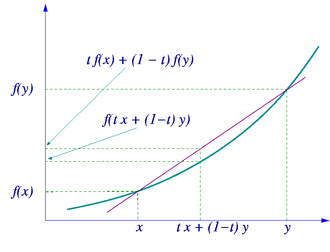
\includegraphics{images/convex_function_graph.png}
			\caption{Illustration fonction convexe [image de Wikipédia]}
			\label{fig:convexe_graph}
		\end{figure}
	
	
	
		
		\paragraph*{Définition : (Fonction convexe)}
		Une fonction $f$ d'un intervalle réel $I \in \mathcal{C}$ est dite fonction convexe lorsque, $\forall (x,y)$ de $I$ tel que $(x,y) \in \mathcal{C}^2$ et tout $\alpha \in [0, 1]$  on a :
		
				
		\begin{equation}
			f(\alpha x + (1 - \alpha)y) \leq \alpha f(x) + (1 - \alpha)f(y)
			\label{eq_convexe-1}
		\end{equation}
		et si
		\begin{equation}
			f(\alpha x + (1 - \alpha)y) < \alpha f(x) + (1 - \alpha)f(y)
			\label{eq_convexe-2}
		\end{equation}
		on dit que la fonction est strictement convexe dans $\mathcal{C}$,  \cite[voir dans][page:45]{jtshiman:2021}\\\\
		Exemple \cite{jtshiman:2021}: 
		\begin{itemize}
			\item[--] La fonction $ f(x) = x^2$ est convexe. 
			\item[--] La fonction $ f(x) = x^T x$ est convexe.
			\item[--] La fonction $ f(x) = x^T Ax$ est convexe, ssi A est symétrique semi-définie positive.
		\end{itemize}
	
		%\subsection{Extrema}	
		\paragraph*{Propriété d'une fonction dérivable : } (Extremum local) 
		Parmi les propriétés de dérivabilité il existe une qui est mise en relation avec l'effect qu'une fonction doit être convexe. énoncé ci-dessous \cite[voir dans][page:212]{coulombeau2013math}.\\
		\begin{list}{+}{Soit $I \rightarrow  \mathbb{R} $ une fonction et $a$ un point de $I$.}
			\item  {On dit que $m$ est un \textbf{minimum local} de $f$ s'il existe $a > 0$ tel que $m$ soit le minimum de $f$ restreinte à $I \cap ] a-\alpha, a + \alpha [$. }
			\item On dit que $M$ est un \textbf{maximum local} de $f$ s'il existe $a > 0$ tel que $M$ soit le maximum de $f$ restreinte à $I \cap ] a-\alpha, a + \alpha [$. 
		\end{list} 
		
		Donc nous pouvons dire qu'une fonction convexe à un unique point minimum.
		
		 
		\subsubsection{Développement limité}\label{sec:dev_lim}
		En physique et en mathématiques, un développement limité (noté DL) d'une fonction en un point est une approximation polynomiale de cette fonction au voisinage de ce point, c'est-à-dire l'écriture de cette fonction sous la forme de la somme d'une fonction polynomiale et d'un reste négligeable au voisinage du point considéré \cite{coulombeau2013math}.
		
		Soit $f$ une fonction à valeurs réelles définie sur un intervalle $I$, et $x_0 \in I$. On dit que $f$ admet un développement limité d'ordre $n^2$ (abrégé par $DL_n$) en $x_0$, s'il existe $n + 1$ réels $a_0, a_1, \dots, a_n$  tels que la fonction ${\displaystyle R:I\to \mathbb {R} }$ définie par :
		$${\displaystyle f(x)=a_{0}+a_{1}(x-x_{0})+a_{2}(x-x_{0})^{2}+\dots+a_{n}(x-x_{0})^{n}+R(x)=\sum _{i=0}^{n}a_{i}(x-x_{0})^{i}+R(x)}$$
		vérifie : $R(x)$ tend vers $0$ lorsque $x$ tend vers $x_0$, et ce plus rapidement que le dernier terme de la somme, c'est-à-dire que :
		$$
			\lim _{{x\rightarrow x_{0}}}{\frac{R(x)}{(x-x_{0})^{n}}}=0. 
		$$
		
		La fonction reste $R(x)$ vérifiant ceci est notée $o((x – x0)^n)$ (selon la notation de Landau). On écrit donc :
		
		$$
			f(x)= \sum _{i=0}^{n}a_{i}(x-x_{0})^{i}+R(x) =\sum _{{i=0}}^{n}a_{i}(x-x_{0})^{i}+o((x-x_{0})^{n})
		$$
		
		%\begin{tabular}{r l}
			%\( f(x)\) & \( =\sum _{i=0}^{n}a_{i}(x-x_{0})^{i}+R(x)\) \\
			%& \(=\sum _{{i=0}}^{n}a_{i}(x-x_{0})^{i}+o((x-x_{0})^{n}) \)
		%\end{tabular}
		
		Il est fréquent d'écrire un développement limité en posant $x = x0 + h$ on aura:
		
		
		$$
			f(x_{0}+h)=\sum _{{i=0}}^{n}a_{i}h^{i}+o(h^{n})
		$$
		
		\paragraph*{Conséquences immédiates}
		\begin{itemize}
			\item Si $f$ admet un $DL_0$ en $x_0$, alors $a_0 = f(x_0)$. \cite{coulombeau2013math}
			\item Si $f$ admet un $DL_n$ en $x_0$, alors elle admet un $DL_k$ en $x_0$ pour tout entier $k < n$ \cite{coulombeau2013math}.
			\item Une condition nécessaire et suffisante pour que f admette un $DL_n$ en $x_0$ est l'existence d'un polynôme $P$ tel que $f(x) = P(x) + o((x – x_0)^n)$ \cite{coulombeau2013math}. S'il existe un tel polynôme $P$, alors il en existe une infinité d'autres, mais un seul d'entre eux est de degré inférieur ou égal à $n$ : le reste de la division euclidienne de $P(X)$ par $(X – x_0)^{n+1}$. On l'appelle la partie régulière, ou partie principale, du $DL_n$ de $f$ en $x_0$. %On identifie parfois, par abus de langage, le $DL_n$ avec sa partie régulière.
		\end{itemize}
		
		
			
		Le théorème de Taylor-Young assure \cite[voir dans][page:241]{coulombeau2013math} qu'une fonction $f$ dérivable n fois au point $x_0$ (avec ${\displaystyle n\geq 1}n\geq 1)$ admet un DLn en ce point :
		
		$$
			{\displaystyle f(x)=f(x_{0})+f'(x_{0})(x-x_{0})+{\frac {f''(x_{0})}{2!}}(x-x_{0})^{2}+\dots +{\frac {f^{(n)}(x_{0})}{n!}}(x-x_{0})^{n}+o((x-x_{0})^{n})}
		$$
		
		soit en écriture abrégée
		$$
			f(x)=\sum _{{i=0}}^{n}{\frac  {f^{{(i)}}(x_{0})}{i!}}(x-x_{0})^{i}+o((x-x_{0})^{n})
		$$
		
		Le développement d'ordre $0$ en $x_0$ revient à écrire que $f$ est continue en $x_0$ :
		
		$$
		{\displaystyle f(x)=f(x_{0})+o((x-x_{0})^{0})=f(x_{0})+o(1)}
		$$
		
		Le développement limité d'ordre 1 en $x_0$ revient à approcher une courbe par sa tangente en $x_0$ on parle aussi d'approximation affine :
		
		$$
		f(x)=f(x_{0})+f'(x_{0})\cdot (x-x_{0})+o(x-x_{0})
		$$
		
		\subsubsection{Différentiabilité au sens de Fréchet} \label{sec:drv_frechet}
			Soient $E$ un espace vectoriel normé, $F$ un espace vectoriel topologique séparé, $f$ une application de $E$ dans $F$ et $a$ un point de $E$. On abandonne la notation des vecteurs par des flèches dans ce paragraphe.
			
			On dit que $f$ est différentiable en $a$ (au sens de Fréchet) s'il existe une application linéaire continue ${\displaystyle L:E\to f}$ telle que :
			$$
			\forall h\in E\quad f(a+h)=f(a)+L(h)+o\left(\|h\|\right)
			$$
			ou, de manière équivalente :
			
			$$
			\lim _{h\to 0}{\frac {f(a+h)-f(a)-L(h)}{\|h\|}}=0.
			$$
			
			Une telle application linéaire $L$ est alors unique.
			L’opérateur $L$ est appelé différentielle de Fréchet (ou F-différentielle, ou Fréchet-différentielle) de $f$ au point $a$, et $f$ est dite Fréchet-différentiable (ou différentiable, ou différentiable au sens de Fréchet) au point $a$. La différentielle de $f$ au point $a$ est souvent notée $Df(a)$, la notation
			$f'(a)$ est aussi utilisée.
	\subsection{Fonctions dérivables}
		
	
	\subsubsection{Gradient}\label{sec:gradient}
		\paragraph*{Définition:}Le gradient d'une fonction de plusieurs variables en un certain point est un vecteur qui caractérise la variabilité de cette fonction au voisinage de ce point. Défini en tout point où la fonction est différentiable, il définit un champ de vecteurs, également dénommé gradient. Le gradient est la généralisation à plusieurs variables de la dérivée d'une fonction d'une seule variable.%\\ \\
		\paragraph*{Définition mathématique :} Dans un système de coordonnées cartésiennes, le gradient d'une fonction {$ f(x_{1},x_{2},\dots ,x_{n}$)} est le vecteur de composantes {$ \partial f/ \partial x_{i}\ (i=1,2,\dots ,n)$}, c'est-à-dire les dérivées partielles de $f$ par rapport aux coordonnées \cite{jtshiman:2021}.
		$${\nabla f(x)={
				\begin{bmatrix}
					{\frac {\partial f(x)}{\partial x_{1}}}\\
					\vdots \\
					{\frac {\partial f(x)}{\partial x_{n}}}
				\end{bmatrix}}} \in \mathbb{R}^n $$
		\pagebreak
		\paragraph*{Gradient sous forme de développement limité:}
		\textit{Si une application admet un gradient en un point, alors on peut écrire ce développement limité du premier ordre (voir le point \ref{sec:dev_lim})}.
		
		$${ 
			f(x+h)=f(x)+\langle \nabla f(x)\mid h\rangle +o(h) 
		}$$ 
		ou 
		$$ {  
			f(x-h)=f(x)-\langle \nabla f(x)\mid h\rangle +o(h)
		}$$
		\textit{Numériquement, il est très intéressant de faire ensuite la demi-différence des deux développements pour obtenir la valeur du gradient et on note que celui-ci ne dépend pas en fait de la valeur de la fonction au point $x : f (x)$. Cette formule a l'avantage de tenir compte des gradients du 2e ordre et est donc beaucoup plus précise et numériquement robuste. L'hypothèse est, en pratique, de connaitre les valeurs "passé" et "futur" de la fonction autour d'un petit voisinage du point $x$}.\\
		\paragraph*{Définition numérique:}
		Une fonction multivariée (à variable vectorielle)
		$ f(x)	: \mathbb{R}^n \rightarrow \mathbb{R} : x \rightarrow f(x) $ définie sur un ouvert $O \in \mathbb{R}^n$ est dite dérivable (au sens de Fréchet, voir le point \ref{sec:drv_frechet}) en $x$ ssi il existe un vecteur noté $\nabla f(x) \in \mathbb{R}^n$ tel que
		\begin{equation}
			f(x+h) = f(x) + \nabla f(x)^{T}h + o(||h||)
		\end{equation}
		
		$\nabla f(x) \in \mathbb{R}^n$ et où l’on a posé que le reste $o(||h||) = ||h||\epsilon (h) \in \mathbb{R}^n$, avec $h \in \mathbb{R}^n$ 
		\begin{center}
			$\epsilon (h): \mathbb{R}^n\rightarrow \mathbb{R}, \hspace{1 cm} \lim\limits_{||h|| \rightarrow 0} \epsilon(h)=0$.
		\end{center} 
		Le vecteur $\nabla f(x)$ est unique et s’appelle \textbf{gradient} de $f(x)$ en $x$.
		Le gradient s’adresse aux fonctions scalaires à variables vectorielles.
		\paragraph*{A propos de la notation $\textbf{o(||h||)}$:}
		La notation de Landau $o(||h||)$ traduit le comportement d’une fonction de $h$ qui [est ??] tend vers $0$ d’un ordre de grandeur plus vite que $||h||$.\\\\
		Elle est infiniment plus petit que $h$ dans le voisinage de $0$
		
		
		
			
	\subsubsection{Hessienne}
	\paragraph*{Définition mathématique:}
	Étant donnée une fonction ${f}$ à valeurs réelles
	
	$${ f:\mathbb{R}^{n}\to \mathbb {R} ;(x_{1},...,x_{n})\mapsto f(x_{1},...,x_{n})}$$
	dont toutes les dérivées partielles secondes existent, le coefficient d'indice ${ i,j}$ de la \textbf{matrice hessienne\footnote{En mathématiques, la matrice hessienne (ou simplement la hessienne) d'une fonction numérique $f$ est la matrice carrée, notée $H(f)$, de ses dérivées partielles secondes.}} ${H(f)}$ vaut ${H_{ij}(f)={\frac {\partial ^{2}f}{\partial x_{i}\partial x_{j}}}}$.\\
	Autrement dit,
	$$
	{ H(f)={
		\begin{bmatrix}{
			\frac {\partial ^{2}f}{{\partial x_{1}}^{2}}}&{\frac {\partial ^{2}f}{\partial x_{1}\partial x_{2}}}&\cdots &{\frac {\partial ^{2}f}{\partial x_{1}\partial x_{n}}}\\
			{\frac {\partial ^{2}f}{\partial x_{2}\partial x_{1}}}&{\frac {\partial ^{2}f}{{\partial x_{2}}^{2}}}&\cdots &{\frac {\partial ^{2}f}{\partial x_{2}\partial x_{n}}}\\
			\vdots &\vdots &\ddots &\vdots \\
			{\frac {\partial ^{2}f}{\partial x_{n}\partial x_{1}}}&{\frac {\partial ^{2}f}{\partial x_{n}\partial x_{2}}}&\cdots &{\frac {\partial ^{2}f}{{\partial x_{n}}^{2}}}
		\end{bmatrix}}} .
	$$
	
	\paragraph*{Définition numérique:}
	Supposons que $f : \mathbb{R}^{n} \to \mathbb{R}$ définie sur un ouvert $\mathcal{O} \in \mathbb{R}^{n}$. La fonction $f(x)$ est dite 2
	fois continûment dérivable (au sens de Fréchet??) si en tout $x \in \mathcal{O}$ on a
	
	\begin{equation}
		f(x + h) = f(x)+\nabla f(x)^Th + \frac{1}{2}h^T\nabla^2f(x)h+o(||h||^2)
	\end{equation}
	avec$\nabla f(x)\in \mathbb{R}^{n\times n}$ et où on a posé que le reste 
	$ o(||h||^2) =||h|| \epsilon(h) \in \mathbb{R} $ avec 
	$\lim\limits_{||h|| \to 0} \epsilon(h) = 0 $
	La matrice carrée symétrique $\nabla^2 f(x)$ appelée \textbf{Hessien} de $f(x)$ en $x$. Remarque :
	
	$$
		\lim\limits_{||h|| \to h} \frac{o(||h||^2)}{||h||} = 0  \in \mathbb{R}
	$$
	La Hessienne s’adresse aux fonctions scalaires à variables vectorielles.
			
	\subsubsection{Jacobienne}
	\paragraph*{Définition mathématique:}
	Soit F une fonction d'un ouvert de $\mathbb{R}^{n}$ à valeurs dans $\mathbb{R}^{m}$ ($F:\mathbb{R}^{n}\to \mathbb {R}^{m}$). Une telle fonction est définie par ses $m$ fonctions composantes à valeurs réelles :
	
	$$ 
	{ F:
		{\begin{pmatrix}
			x_{1}\\\vdots \\
			x_{n}
		\end{pmatrix}}
		\longmapsto 
		{\begin{pmatrix}
			f_{1}(x_{1},\dots ,x_{n})\\
			\vdots \\f_{m}(x_{1},\dots ,x_{n})
		\end{pmatrix}}}.
	$$
	Les dérivées partielles de ces fonctions en un point $M$, si elles existent, peuvent être rangées dans une matrice à $m$ lignes et $n$ colonnes, appelée \textbf{matrice jacobienne\footnote{En analyse vectorielle, la matrice jacobienne est la matrice des dérivées partielles du premier ordre d'une fonction vectorielle en un point donné.}} de $F$ :
	$$
	J_{F}\left(M\right)={
		\begin{pmatrix}
			{\dfrac {\partial f_{1}}{\partial x_{1}}}&\cdots &{\dfrac {\partial f_{1}}{\partial x_{n}}}\\
			\vdots &\ddots &\vdots \\
			{\dfrac {\partial f_{m}}{\partial x_{1}}}&\cdots &{\dfrac {\partial f_{m}}{\partial x_{n}}}
		\end{pmatrix}}.
	$$
	
	La case sur la ligne i et la colonne j contient ${\displaystyle {\frac {\partial f_{i}}{\partial x_{j}}}}$ qui est la dérivée partielle de fi selon la variable xj. Cette matrice est notée :
	
	$${\displaystyle J_{F}\left(M\right),\qquad {\frac {\partial \left(f_{1},\ldots ,f_{m}\right)}{\partial \left(x_{1},\ldots ,x_{n}\right)}}\qquad {\text{ou}}\qquad {\frac {\mathrm {D} \left(f_{1},\ldots ,f_{m}\right)}{\mathrm {D} \left(x_{1},\ldots ,x_{n}\right)}}}$$
	
	Pour $i = 1, … , m,$ la i-ème ligne de cette matrice est la transposée du vecteur \textbf{gradient} (voir le point \ref{sec:gradient}) au point $M$ de la fonction $f_i$, lorsque celui-ci existe. La matrice jacobienne est également la matrice de la différentielle de la fonction, lorsque celle-ci existe.
	\paragraph*{Définition numérique:}
	
	Soit $f(x) : \mathbb{R}^n \to \mathbb{R}^m$ définie sur un ouvert $ \mathcal{O} \subset \mathbb{R} $. On dit que $f(x)$ est dérivable
	(au sens de Fréchet) en $x$, si chacune des composantes $f_i(x)$ est dérivable  en $x$. On a alors
	
	\begin{equation}
		f(x + h) = f(x) + D_f (x)h + o(||h||)
	\end{equation}
	avec $D_f (x) \in  \mathbb{R}^{n \times m} $ et/où $ o(||h||)=||h|| \epsilon(h) \in \mathbb{R}^m $ avec $\lim\limits_{||h|| \to 0} \epsilon(h) = 0 $.
	Remarque :
	$$
		\lim\limits_{||h|| \to h} \frac{o(||h||^2)}{||h||} = 0  \in \mathbb{R}
	$$
	
	Soient 
	$x = 
		\begin{bmatrix}
			x_1 & x_2& \cdots & x_n
		\end{bmatrix}^{T}
		\in \mathbb{R}^n $ et $ 
	f(x) = 
		\begin{bmatrix}
			f_1(x) & f_2(x)& \cdots & f_n(x)
		\end{bmatrix}^{T} \in \mathbb{R}^m
	$
	
	$$
	D_f\left(x\right)={
		\begin{bmatrix}
		{\dfrac {\partial f_{1}(x)}{\partial x_{1}}}&\cdots &{\dfrac {\partial f_{1}(x)}{\partial x_{n}}}\\
		\vdots &\ddots &\vdots \\
		{\dfrac {\partial f_{m}(x)}{\partial x_{1}}}&\cdots &{\dfrac {\partial f_{m}(x)}{\partial x_{n}}}
		\end{bmatrix}}
		=
		\begin{bmatrix}
		\nabla f_1(x)^T \\ \nabla f_2(x)^T\\ \vdots \\ \nabla f_m(x)^T
		\end{bmatrix}
		\in  \mathbb{R}^{n \times m},
	$$
	La matrice $D_f (x) \in  \mathbb{R}^{n \times m} $ est appelée \textbf{Jacobienne} de f(x) en x.
	La Jacobienne s’adresse aux fonctions vectorielles à variables vectorielles.
	
	
	
		
		
	\begin{description}
		\item[Note:] Lorsque $m=1$ (m : nombre des lignes), la Jacobienne est la même que le gradient car il s'agit d'une généralisation du gradient.
	\end{description}
	
		
		
		
	\section{Statistique \& probabilité}

	\subsection{Échantillonnage (Statistique)}
	
	En statistiques, l'échantillonnage est la sélection d'un sous-ensemble (un échantillon statistique ) d'individus au sein d'une population statistique pour estimer les caractéristiques de l'ensemble de la population. 
	
	
	Sur un échantillon, on peut calculer différents paramètres statistiques de position (moyenne, etc.) ou de dispersion (écart type, etc.) issus de la statistique descriptive, de la même manière que l'on peut déterminer des paramètres statistiques d'une population par son recensement exhaustif.
	
	On peut également déduire des propriétés de la population à partir de celles de l'échantillon par inférence statistique. D'après la loi des grands nombres, plus la taille de l'échantillon augmente, plus ses propriétés seront proches de celle de la population. En particulier, on peut estimer une probabilité sur les individus d'une population par la fréquence observée sur un échantillon si sa taille est suffisamment grande. 
	
	Cette méthode présente plusieurs avantages : une étude restreinte sur une partie de la population, un moindre coût, une collecte des données plus rapide que si l'étude avait été réalisé sur l'ensemble de la population, la réalisation de contrôles destructifs, etc.
	
	\begin{list}{$\triangleright$ }{On peut procéder de différentes manières pour collecter les données de l'échantillon, il existe en effet plusieurs méthodes d'échantillonnage \cite{sarndal2003model} :}
		%\textbf
		\item  \textbf{Échantillonnage aléatoire et simple }: le tirage des individus de l'échantillon est aléatoire, c'est-à-dire que chaque individu a la même probabilité d'être choisi, et simple, c'est-à-dire que les choix des différents individus sont réalisés indépendamment les uns des autres.
		%L'échantillonnage aléatoire simple peut être vulnérable aux erreurs d'échantillonnage car le caractère aléatoire de la sélection peut donner un échantillon qui ne reflète pas la composition de la population. 
		
		\item  \textbf{Échantillonnage systématique }: le premier individu est choisi de manière aléatoire, puis les suivants sont déterminés à intervalle régulier. Par exemple, dans un verger, on choisit au hasard le 7e pommier, puis les 27e, 47e, 67e, etc.
		
		\item  \textbf{Échantillonnage stratifié }: on subdivise la population en plusieurs parties avant de prendre l'échantillon1.
		
		\item \textbf{Échantillonnage par quotas }: la composition de l'échantillon doit être représentative de celle de la population selon certains critères jugés particulièrement importants. On utilise cette méthode pour réaliser les sondages d'opinions.
	\end{list}

	
	\subsubsection{La collecte de données }
	
	La collecte de données est le processus de collecte et de mesure des informations sur des variables ciblées dans un système établi, qui permet ensuite de répondre aux questions pertinentes et d'évaluer les résultats.
	
	\begin{list}{--}{Une bonne collecte de données implique :}
		\item Suivre le processus d'échantillonnage défini
		\item Garder les données dans l'ordre du temps
		\item Noter les commentaires et autres événements contextuels
		\item Enregistrement des non-réponses
	\end{list}
	
	\paragraph*{Erreur d'échantillonnage :}
	Dans les statistiques, les erreurs d'échantillonnage se produisent lorsque les caractéristiques statistiques d'une population sont estimées à partir d'un sous-ensemble, ou échantillon, de cette population. Étant donné que l'échantillon n'inclut pas tous les membres de la population, les statistiques de l'échantillon (souvent appelées estimateurs), telles que les moyennes et les quartiles, diffèrent généralement des statistiques de l'ensemble de la population (appelées paramètres ). La différence entre la statistique d'échantillon et le paramètre de population est considérée comme l'erreur d'échantillonnage \cite{sarndal2003model}. 
	
	
	
		
	\subsection{Analyse bayésienne}
		La statistique bayésienne est une théorie dans le domaine des statistiques basée sur l' interprétation bayésienne de la probabilité où la probabilité exprime un degré de croyance en un événement. Le degré de croyance peut être basé sur des connaissances antérieures sur l'événement, telles que les résultats d'expériences précédentes, ou sur des croyances personnelles sur l'événement. Cela diffère d'un certain nombre d'autres interprétations de la probabilité , telles que l' interprétation fréquentiste qui considère la probabilité comme la limite de la fréquence relative d'un événement après de nombreux essais [??].
		
		Les statistiques bayésiennes portent le nom de Thomas Bayes\footnote{Thomas Bayes était un Anglais statisticien , philosophe et ministre presbytérien qui est connu pour la formulation d' un cas spécifique du théorème qui porte son nom : théorème de Bayes.}, qui a formulé un cas spécifique du théorème de Bayes dans un article publié en 1763.
		
		
		
		\begin{thm}[Théorème de Bayes] Le théorème de Bayes est utilisé dans les méthodes bayésiennes pour mettre à jour les probabilités, qui sont des degrés de croyance, après avoir obtenu de nouvelles données. Compte tenu de deux événements $A$  et $B$, la probabilité conditionnelle de $A$ étant donné que $B$ est vrai s'exprime comme suit  :
			\begin{equation}
				\mathbb{P}(A|B) = \frac{\mathbb{P}(B|A) \mathbb{P}(A)}{\mathbb{P}(B)}
			\end{equation}
			
		\end{thm}
	
		où $\mathbb{P}(B) \ne 0$ Bien que le théorème de Bayes soit un résultat fondamental de la théorie des probabilités , il a une interprétation spécifique dans les statistiques bayésiennes \cite[][]{antoine2018apprentissage}.

		
%#############################################################################
%
%              						CHAPTER 
%
%#############################################################################


%\textcolor{cyan}{\chapter{Apprentissage automatique : Modélisation et Classification }}
	%\section{Généralité}
	\section{Généralité sur la modélisation et la classification }
	\subsection{Les ingrédients d'apprentissage}
	Résoudre un problème d'apprentissage, c'est d'abord le comprendre, c'est-à-dire discuter longuement avec les experts du domaine concerné pour identifier quelles sont les "entrées", les  "sorties" ou résultats désirés, les connaissances disponibles, les particularités des données, par exemple: valeurs manquantes, taux de bruit dans les mesures des attributs de description, proportions des classes, stationnarité ou pas de l'environnement. 
	C'est aussi réaliser un gros travail de \textit{préparation des données}: nettoyage, ré-organisation, enrichissement, intégration avec d'autres sources de données, etc. Ces étapes de compréhension du problème, de préparation des données, de mise au point du protocole d'apprentissage et des mesures d'évaluation des résultats, prennent, et de loin, la plus grande partie du temps pour (tenter de) résoudre un problème d'apprentissage \cite{antoine2018apprentissage}. 
	Nous avons toujours tendance à largement sous-estimer ces étapes et à vouloir se concentrer uniquement sur la phase excitante de l'essai de méthodes d'apprentissage sur des données supposées bonnes à la consommation. 
	%\subsubsection{Algorithme qui apprennent}
	
	
	\subsection{Modélisation}\label{sec:modelisation}
	La modélisation est la conception et l'utilisation d'un \textit{modèle}. Selon son objectif et les moyens utilisés, la modélisation est dite mathématique, géométrique, 3D, empirique, etc. 
	En informatique, la modélisation permet de concevoir l'architecture globale d'un système d'information, ainsi que l'organisation des informations à l'aide de la modélisation des données ;
	
	\paragraph*{Modèle (informatique):} En informatique, un modèle a pour objectif de structurer les informations et activités d'une organisation : données, traitements, et flux d'informations entre entités.
	
	\paragraph*{Modèle (mathématique):} Un modèle mathématique est une description d'un système utilisant des concepts et un langage mathématiques.
	
	Un modèle peut aider à expliquer un système et à étudier les effets de différents composants, et à faire des prédictions sur le comportement.
	
	\subsubsection{Modèles non paramétriques}
	
	
	\Eg: Prenons l'exemple de données décrites dans l'espace d'entrée $\mathcal{X} = \mathbb{R}^n$ avec $n$ variables réelles et supposons-les étiquetées par $\times$ ou par $\bullet$. On cherche donc une fonction de décision $h$, appelée hypothèse ou modèle, telle qu'elle soit capable d'étiqueter toute entrée 
	$x \in \mathcal{X}, h: x \rightarrow \{\times,\bullet\}$. Reste à définir l'espace des hypothèses ou modèles $\mathcal{H}$ que l'on est prêt à considérer.
	
	Toujours en considérant le problème de prédiction basique (présenté ci-dessus), on pourrait définir une hypothèse par une procédure qui examine les trois plus proches voisins du point à étiqueter $x$ et qui choisit l'étiquette majoritaire parmi ces trois points pour étiqueter $x$. Il n'y a évidemment plus de paramètres pour définir les modèles possibles \cite[p. 24]{antoine2018apprentissage}.
	
	Un \textbf{modèle non paramétrique} est construit selon les informations provenant des données. Dans \cite{antoine2018apprentissage} \cite[p. 120]{bishop2006pattern} il est expliqué que : La régression non paramétrique exige des tailles d'échantillons plus importantes que celles de la régression basée sur des modèles paramétriques parce que les données doivent fournir la structure du modèle ainsi que les estimations du modèle.
	
	Un \textbf{modèle paramétrique} est, s'il est approximativement valide, plus puissant qu'un modèle non paramétrique, produisant des estimations d'une fonction de régression qui ont tendance à être plus précises que ce que nous donne l'approche non paramétrique \cite{matloff2017statistical}. Cela devrait également se traduire par une prédiction plus précise. 
	
	
	
	\begin{list}{--}{Selon \cite[A. Cornuéjols][]{antoine2018apprentissage}, nous pouvons construire un modèle d'apprentissage, ou l'espaces des hypothèses d'apprentissage, par: }
		\item La classification
		\item La régression
		\item Les distributions de probabilités
		\item Les arbres de décisions
		\item Les réseaux bayésiens 
		\item Etc.
	\end{list}

	La table suivante présente d'abord les qualités des différentes représentations des hypothèses en fonction des critères cités ci-dessus.
	

	%\parbox[t]{2mm}{\multirow{3}{*}{\rotatebox[origin=c]{90}{rota}}} 
	\begin{center}
		\begin{tabular}{l|cccccc}
			& \rotatebox[origin=c]{90}{Fonctions séparatrices}
			&  \rotatebox[origin=c]{90}{Distributions de probabilités}
			& \rotatebox[origin=c]{90}{Arbres de décision }
			& \rotatebox[origin=c]{90}{Hiérarchies de concepts}
			& \rotatebox[origin=c]{90}{Réseaux bayésiens } 
			& \rotatebox[origin=c]{90}{Chaînes de Markov}\\
			\hline
			
			Concept & $\surd$ &$\surd$ &$\surd$ &$\surd$ & --&-- \\
			Classes multiples &$\surd$ & $\surd$ &$\surd$ &$\surd$ &--&-- \\
			Ontologies & --&-- & $\surd$&$\surd$ & --&-- \\
			Régression &-- &$\surd$ & $\surd$&-- &-- &-- \\
			Évolutions temporelles &-- &$\surd$ &-- &-- &-- & $\surd$\\
			Apprentissage non supervisé & $\surd$ &$\surd$ &$\surd$ &$\surd$ &-- &-- \\
			Données continues & $\surd$ &$\surd$ &$\surd$ &-- &-- &$\surd$  \\
			Connaissances relationnelles  & & & & $\surd$  & $\surd$  &-- \\
			Degré de certitude &-- &$\surd$ &-- &-- &$\surd$ &$\surd$ \\
			Degré d'imprécision &-- &$\surd$ &-- &-- &$\surd$ &-- \\
			Transparence, intelligibilité &-- &-- &-- &$\surd$ &$\surd$ &$\surd$ \\
			%& & & & \\
			%& & & & \\
			
			
		\end{tabular}
	\end{center}

	
	
	\subsubsection{Entraînement du modèle}
	
	Tout modèle, où toutes les informations nécessaires ne sont pas disponibles, contient certains paramètres qui peuvent être utilisés pour adapter le modèle au système qu'il est censé décrire. Si la modélisation est effectuée par un réseau de neurones artificiels ou un autre apprentissage automatique, l'optimisation des paramètres est appelée \textbf{entraînement} (en anglais : \textbf{training}), tandis que l'optimisation des hyperparamètres du modèle est appelée \textbf{réglage} (en anglais: \textbf{tuning}) et utilise souvent la validation croisée [??]. Dans une modélisation plus conventionnelle à travers des fonctions mathématiques explicitement données, les paramètres sont souvent déterminés par ajustement de courbe (voir le point ??).
	
	
	Une partie cruciale du processus de modélisation consiste à évaluer si oui ou non un modèle mathématique donné décrit un système avec précision. Il peut être difficile de répondre à cette question car elle implique plusieurs types d'évaluation différents.
	
	????
	Un modèle de régression linéaire ajusté peut être utilisé pour identifier la relation entre une seule variable prédictive $x_j$ et la variable de réponse $y$ lorsque toutes les autres variables prédictives du modèle sont "maintenues fixes". Plus précisément, l'interprétation de $\beta_j$ est la variation attendue de $y$ pour une variation d'une unité de $x_j$ lorsque les autres covariables sont maintenues fixes, c'est-à-dire la valeur attendue de la dérivée partielle de $y$ par rapport à $x_j$. Ceci est parfois appelé l'effet unique de $x_j$ sur $y$. En revanche, l'effet marginal de $x_j$ sur $y$ peut être évalué à l'aide d'un coefficient de corrélation ou d'un simple modèle de régression linéaire reliant uniquement $x_j$ à $y$; cet effet est la dérivée totale de $y$ par rapport à $x_j$.

	\section{Régression Linéaire}
	
	L'algorithme d'apprentissage automatique est défini comme un algorithme capable d'améliorer les performances d'un programme informatique à certaines tâches via l'expérience est quelque peu abstraite. Pour rendre cela plus concret, Une des méthode d'apprentissage automatique basique est \emph{la régression linéaire} \cite{goodfellow2016deep}.
	
	Dans la modélisation statistique, l'analyse de régression est un ensemble de processus statistiques permettant d'estimer les relations entre une variable dépendante et une ou plusieurs variables indépendantes [??].\\
	En statistique, la régression linéaire est une approche linéaire pour modéliser (voir le point \ref{sec:modelisation}) la relation entre une réponse scalaire et une ou plusieurs variables explicatives (également appelées variables dépendantes et indépendantes). Le cas d'une variable explicative est appelé régression linéaire simple; pour plus d'un, le processus est appelé régression linéaire multiple.
	
	Dans la régression linéaire, les relations sont modélisées à l'aide de \textit{fonctions prédictives}\footnote{En statistique et en apprentissage automatique, une fonction de prédicteur linéaire est une fonction linéaire d'un ensemble de coefficients et de variables explicatives, dont la valeur est utilisée pour prédire le résultat d'une variable dépendante.} linéaires dont les paramètres de modèle inconnus sont estimés à partir des données \cite{matloff2017statistical}. De tels modèles sont appelés modèles linéaires.
	
	La régression linéaire a de nombreuses utilisations pratiques. Si l'objectif est la prédiction, la prévision ou la réduction des erreurs, la régression linéaire peut être utilisée pour ajuster un modèle prédictif à un ensemble de données observées de valeurs de la réponse et de variables explicatives \cite{darlington2016regression}. Après avoir développé un tel modèle, si des valeurs supplémentaires des variables explicatives sont collectées sans valeur de réponse d'accompagnement, le modèle ajusté peut être utilisé pour faire une prédiction de la réponse.
	
	Dans ce type de tâche, le programme informatique est invité à prédire une valeur numérique à partir d'une entrée donnée. Pour résoudre cette tâche, l'algorithme d'apprentissage est invité à sortir une fonction $f : \mathbb{R}^n \rightarrow \mathbb{R}$. Ce type de tâche est similaire à la \textbf{classification}, sauf que le format de sortie est différent \cite{goodfellow2016deep}.
	
	
	
	
	\subsection{Le problème de la régression linéaire}
		On appelle problèmes de régression de tels problèmes, dans lesquels la sortie est numérique, généralement un vecteur de réels, supposé dépendre de la valeur d'un certain nombre de facteurs en entrée.
		
		Le vecteur d'entrée $x = (1,2,...,x)^T$ est souvent appelé variable indépendante, tandis que le vecteur de sortie $y$ est appelé variable dépendante. On formalise le problème en supposant que la sortie résulte de la somme d'une fonction déterministe $f$ de l'entrée et d'un bruit aléatoire :
		\begin{equation}
			y = f(x) + \epsilon
		\end{equation}
	
		où $f(x)$ est la fonction inconnue que nous souhaitons approcher par un estimateur $h(x|w)$, où $h$ est défini à l'aide d'un vecteur $w$ de paramètres.\\
		Si l'on suppose que le bruit $\epsilon$ est un phénomène gaussien de moyenne nulle et de variance constante $\sigma^2$, c'est-à-dire $ \epsilon = \mathcal{N}(0,\sigma^2)$, alors, en plaçant notre estimateur $h(\cdot)$ à la place de la fonction inconnue, on devrait avoir la densité conditionnelle réelle $p(y|x)$ vérifiant :
		\begin{equation}
			p(y|x) = \mathcal{N}(h(x|w),\sigma^2)
		\end{equation}
		
		On peut estimer le vecteur de paramètres $w$ grâce au principe de maximisation de la vraisemblance. On suppose que les couples $(y_t, y_t)$ de l'échantillon d'apprentissage sont tirés par tirages indépendants d'une distribution de probabilités jointes inconnue $p(x, y)$, qui peut s'écrire :
		
		$$
			p(y|x) = p(y|x)p(x)
		$$
		où $p(y|x)$ est la probabilité de la sortie étant donnée l'entrée et $p(x)$ est la densité de probabilité sur les entrées.
		
		\cite{matloff2017statistical}
		
	%%%\subsubsection*{La régression non linéaire ou multiple}
		%\lipsum[2]
	\subsection{Le cas de la régression générale}
		La plupart des modèles de régression proposent que $Y_{i}$ est une fonction de $X_{i}$ et $\beta$, avec $\epsilon_{i}$ représentant un terme d'erreur additif qui peut remplacer des déterminants non modélisés de $Y_{i}$ ou bruit statistique aléatoire :
		\begin{equation}
			{\displaystyle Y_{i}=f(X_{i},\beta )+\epsilon_{i}}
		\end{equation}
	
	L'objectif est d'estimer la fonction ${\displaystyle f(X_{i},\beta )}$ qui correspond le mieux aux données.
	
	 Pour effectuer une analyse de régression, la forme de la fonction $f$ doit être spécifié. Parfois, la forme de cette fonction est basée sur la connaissance de la relation entre $Y_{i}$ et $X_{i}$. 
	 Si ces connaissances ne sont pas disponibles, un formulaire souple ou pratique pour $f$ est choisi. Par exemple, une simple régression univariée peut proposer
	 $${\displaystyle f(X_{i},\beta )=\beta _{0}+\beta _{1}X_{i}}$$
	 ou
	 $${\displaystyle Y_{i}=\beta _{0}+\beta _{1}X_{i}+e_{i}}$$
	 être une approximation raisonnable du processus statistique générant les données.
	 
	 Différentes formes d'analyse de régression fournissent des outils pour estimer les paramètres. $\beta$. Par exemple, les moindres carrés trouvent la valeur de $\beta$ qui minimise la somme des carrés des erreurs $${\sum _{i}(Y_{i}-f(X_{i},\beta ))^{2}}$$ 
	 
	 Étant donné un ensemble de données ${\displaystyle \{y_{i},\,x_{i1},\ldots ,x_{ip}\}_{i=1}^{n}}$ de $n$ unités statistiques, un modèle de régression linéaire suppose que la relation entre la variable dépendante $y$ et le vecteur $p$ des régresseurs $x$ est linéaire. Cette relation est modélisée par un terme de perturbation ou une variable d'erreur $\epsilon$ : une variable aléatoire non observée qui ajoute du "bruit" à la relation linéaire entre la variable dépendante et les régresseurs. Ainsi le modèle prend la forme
	 
	$${\displaystyle y_{i}=\beta _{0}+\beta _{1}x_{i1}+\cdots +\beta _{p}x_{ip}+\varepsilon _{i}=\mathbf { x} _{i}^{\mathsf {T}}{\boldsymbol {\beta }}+\varepsilon_{i},\qquad avec \quad i=1,\ldots ,n,}
	$$
	
	Souvent, ces $n$ équations sont empilées et écrites en notation matricielle comme
	
	$$
	{\displaystyle \mathbf {y} =X{\boldsymbol {\beta }}+{\boldsymbol {\varepsilon}},\,}
	$$
	
	où
	
	$
	\mathbf{y} ={\begin{pmatrix}y_{1}\\y_{2}\\\vdots \\y_{n}\end{pmatrix}},\quad
	{\displaystyle 
		X={
			\begin{pmatrix}
				\mathbf {x} _{1}^{\mathsf {T}}\\
				\mathbf {x} _{2}^{\mathsf {T}}\\
				\vdots \\
				\mathbf {x} _{n}^{\mathsf {T}}
			\end{pmatrix}}={
			\begin{pmatrix}
				1&x_{11}&\cdots &x_{1p}\\
				1&x_{21} &\cdots &x_{2p}\\
				\vdots &\vdots &\ddots &\vdots \\
				1&x_{n1}&\cdots &x_{np}
			\end{pmatrix}},} \quad
	{\displaystyle {\boldsymbol {\beta }}={
			\begin{pmatrix}
				\beta _{0}\\
				\beta _{1}\\
				\beta _{2}\\
				\vdots \\
				\beta _{p}
			\end{pmatrix}},\quad 
	{\boldsymbol {\varepsilon }}={
		\begin{pmatrix}\varepsilon _{1}\\
			\varepsilon _{2}\\
			\vdots \\
			\varepsilon _{ n}
		\end{pmatrix}}.}$ \\

	$\mathbf{y}$ est un vecteur de valeurs observées ${\displaystyle y_{i}\ (i=1,\ldots ,n)}$ de la variable appelée variable mesurée ou variable dépendante.
	
	$X$ peut être vu comme une matrice de vecteurs-lignes $\mathbf {x} _{i}$ ou de vecteurs-colonnes à $n$ dimensions $X_{j}$, appelées régresseurs, variables explicatives, variables d'entrée, variables prédictives ou variables indépendantes. La matrice $X$ est parfois appelée la matrice de conception. 
	
	${\boldsymbol {\beta}}$ est un vecteur de paramètre de dimension $(p+1)$, où $\beta _{0}$ est le terme d'interception, s'il n'est inclus dans le modèle ${\boldsymbol {\beta}}$ est de dimension $p$. Ses éléments sont appelés effets ou coefficients de régression. 
	En régression linéaire simple , $p = 1$, et le coefficient est appelé \textbf{pente} de régression.\\
	L'estimation statistique et l'inférence dans la régression linéaire se concentrent sur $\beta$. Les éléments de ce vecteur de paramètres sont interprétés comme les dérivées partielles de la variable dépendante par rapport aux différentes variables indépendantes.
		
	%\subsection{La régression linéaire simple}
		%\lipsum[3]
	%\subsection{La régression linéaire multivarié}
		%\subsubsection{Droite de régression} 
		%\subsubsection{Variance, Covariance, \& Corrélation}
	%\subsection{La fonction prédictif \& d'erreur}
		%\lipsum[1]
	
	
	\section{Régression Logistique}
	\subsection{Le problème de classification}
		Lorem ipsum dolor sit amet, consectetur adipiscing elit, sed do eiusmod tempor incididunt ut labore et dolore magna aliqua.
	\subsection{Le cas séparable }
		Lorem ipsum dolor sit amet, consectetur adipiscing elit, sed do eiusmod tempor incididunt ut labore et dolore magna aliqua.
	\subsection{Le cas non séparable }
	
		\begin{figure}
			\centering
			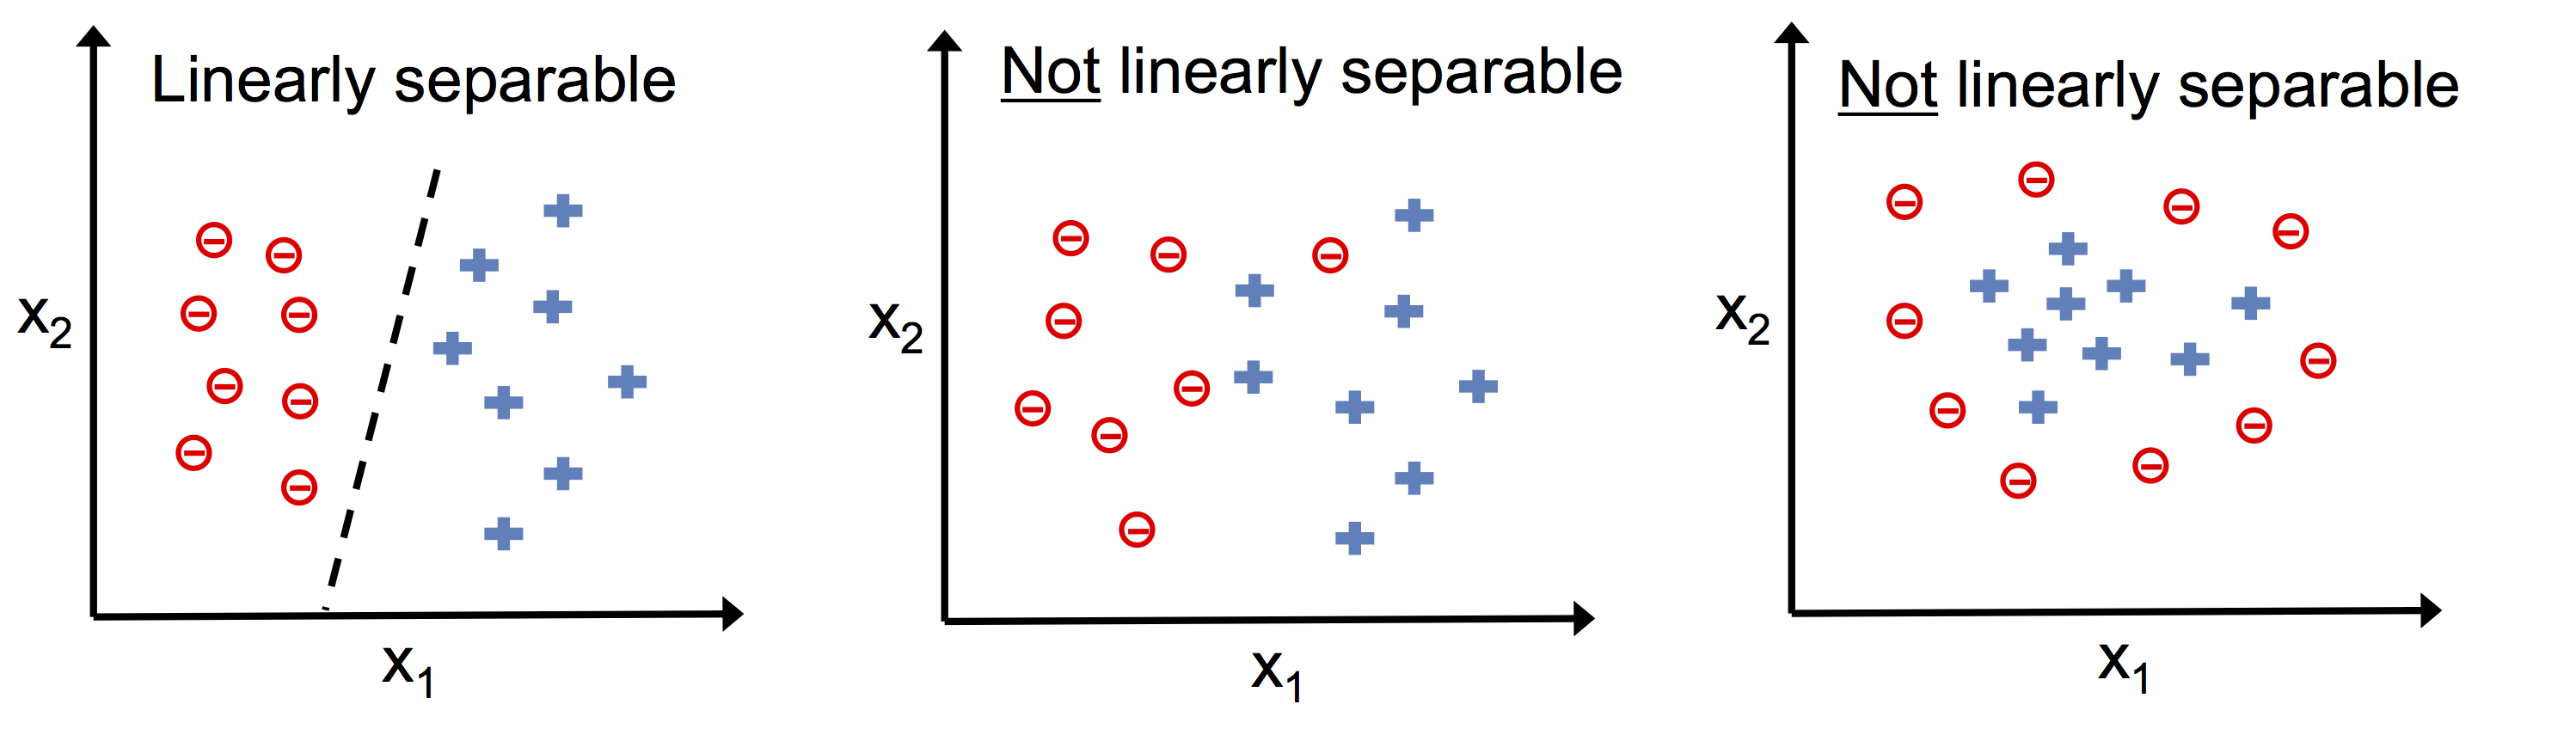
\includegraphics[width=\textwidth]{images/linearly_separable.png}
			\caption{Classes linéairement séparables \cite[image de][page--48]{ml2008python}
		}
			\label{fig:linearly_separable}
		\end{figure}
		\lipsum[3]
	\subsection{Le modèle de la régression logistique }
		\lipsum[1]
		
	\section{Classifications}
	\lipsum[1]
	
	
	\section{Apprentissage profond (Deep Learning)}
	
	\subsection{Perceptron}
	
	\subsection{Neurones}
	\lipsum[1]
	\subsubsection{Réseau neuronal convolutif (CNN)}
	\lipsum[1]
	\subsubsection{Réseau neuronal récurrent (RNN)}
	\lipsum[1]
	
	%\section{Réseaux de neurones}
	
	
	
	%\section{Classificateurs}
	%\lipsum[1]
	

		


%#######################################################################################
%	PART II
%#######################################################################################

%\ctparttext{\centering La méthodologie utilisée parmi tant d’autres, pour entraîner les modèles d’apprentissage automatique (Machine learning Model) de façon optimale. Pour la minimisation de la fonction coût nous utilisons des algorithmes comme SGD, ADAM, ADAGRAD, ADADELTA, ASGD, NAG. Puis faire une étude comparative de leurs performances.} 

%\textcolor{teal}{\part{Méthodologie}}

%#
%

	
\cleardoublepage			


%#############################################################################
%
%              						CHAPTER 
%
%#############################################################################		

%\textcolor{cyan}{\chapter{}}


\textcolor{cyan}{\chapter{Méthode de minimisation des erreurs d'apprentissage}}	
	\section{Collecte des données \& Dataset }
	
	\subsection*{Collecte des données}
	\lipsum[1]
	\lipsum[2]
	\subsubsection{méthode utilisée}
	\lipsum[1]\\
	
	\subsubsection{...}
	\lipsum[1]
	\subsection*{Construction d'un dataset}
	\lipsum[1]
	\subsection*{Choix des technologies}
	\lipsum[1]
	%
	%
	TensorFlow pour entrainer le modèle faire du machine learning
	OpneCV : pour faire du computer vision, la reconnaissance 

	\section{Erreur et fonction coût}
	\lipsum[1]
	\subsection{Erreur d'apprentissage}
	\lipsum[1]
	
	\[\exp(x)=\sum_{k=0}^{\infty}\frac{x^k}{k!}\]
	\lipsum[4]
	\subsubsection{Fonction cout $\ell$ cas de la régression linéaire}
	\lipsum[1]
	\subsubsection{Fonction cout $\ell$ cas  de la classification}
	\lipsum[1]
	
	%\section{Les différent fonction coût}
	\subsection{Erreur quadratique moyenne }
	\lipsum[1] %\cite{bishop2006pattern}
	\subsection{Erreur logarithmique}
	\lipsum[1]
	\begin{figure}[hth]%bth
		\centering
		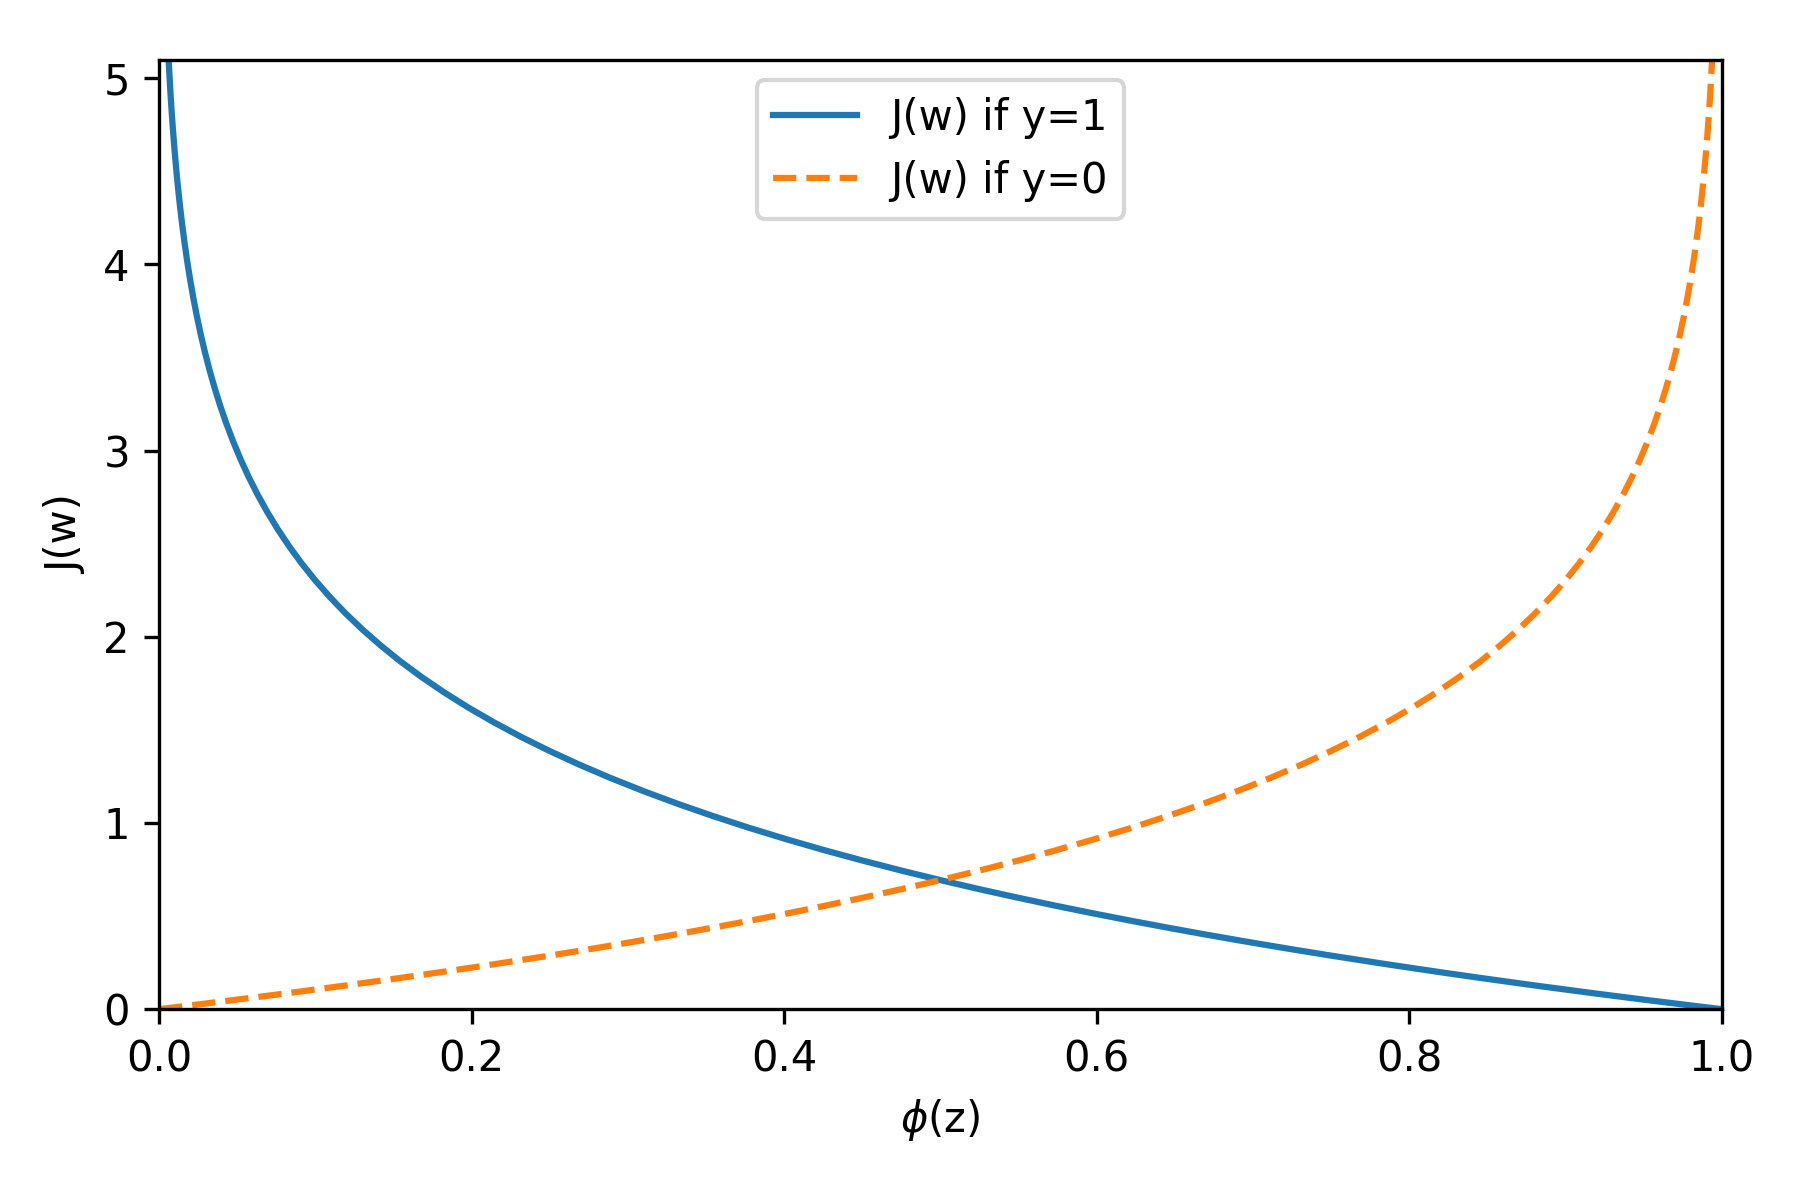
\includegraphics[width=9cm]{images/minimum_log_curve.png}
		\caption{Graphique d'une courbe de régression logistique ajustée aux données $(x_n , y_n)$. \cite[image de]{ml2008python}
		}
		\label{fig:minimum_log_curve}
	\end{figure}
	
	
	
	
	\section{Descente de gradient stochastique}
	Cette section est inspirée des articles écrites par Léon Bottou et al, dans  \cite{bottou2012stochastic} 
	\cite{bottou2010large}
	\cite{framling2004scaled}
	\cite{bottou2018optimization}
	\cite{netrapalli2019stochastic}
	\cite{wijnhoven2010fast}.
	
	\subsection{Descente de gradient (Gradient Descent)}
	
	
	Il a souvent été proposé de minimiser le risque empirique [E] en utilisant la descente de gradient (GD). Chaque itération met à jour les poids w en fonction du gradient de [E] \cite{bottou2012stochastic}.\\
	
	\lipsum[1] \\ 
	
	$$A = \begin{pmatrix}
		x_{11} & x_{12} & x_{13} & \cdots & x_{1n} \\
		x_{21} & x_{22} & x_{23} & \cdots & x_{2n} \\
		\vdots & \vdots & \vdots & \ddots & \vdots \\
		x_{m1} & x_{m2} & x_{m3} & \cdots & x_{mn} 
	\end{pmatrix}$$
	
	
	\lipsum[4]
	\subsubsection{Pourquoi stochastique?}
	Descente de gradient stochastique (SGD) 
	
	L'algorithme de descente de gradient stochastique (SGD) est une simplification drastique. Au lieu de calculer exactement le gradient de E n (f w ), chaque itération estime ce gradient sur la base d'un seul exemple z t pris au hasard \cite{bottou2012stochastic} :
	$$
	{\displaystyle w:=w-\eta \nabla Q(w)=w-{\frac {\eta }{n}}\sum _{i=1}^{n}\nabla Q_{i}(w),}
	$$
	\lipsum[1]	
	\subsection{La convergence de la descente de gradient stochastique}
	\lipsum[1]	
	
	\section{Les optimiseurs SGD}
	\subsection{Perceptron Optimizer}
	
	Le perceptron est un modèle simplifié d'un neurone biologique . Alors que la complexité des modèles de neurones biologiques est souvent nécessaire pour bien comprendre le comportement neuronal, la recherche suggère qu'un modèle linéaire de type perceptron peut produire certains comportements observés dans de vrais neurones.
	
	Un perceptron est une unité de réseau neuronal (un neurone artificiel) qui effectue certains calculs pour détecter des caractéristiques ou une intelligence économique dans les données d'entrée.
	Et aussi en Machine Learnig (apprentissage automatique), le perceptron est un algorithme d'apprentissage supervisé de classificateurs binaires (qui se fait dans la régression logistique). 
	Un classificateur binaire est une fonction qui peut décider si une entrée, représentée par un vecteur de nombres, appartient ou non à une classe spécifique. \cite{freund1999large} Il s'agit d'un type de classificateur linéaire , c'est-à-dire un algorithme de classification qui fait ses prédictions sur la base d'une fonction prédictive linéaire combinant un ensemble de poids avec le vecteur de caractéristiques .
	
	Le premier concept de règle d'apprentissage du perceptron, a été publié par Frank Rosenblatt [??],  basé sur le modèle neuronal MCP(???). 
	
	(F. Rosenblatt, The Perceptron, a Perceiving and Recognizing Automaton. Cornell Aeronautical Laboratory, 1957).
	
	Avec sa règle de perceptron, Rosenblatt a proposé un algorithme qui apprendrait automatiquement les coefficients de poids optimaux qui sont ensuite multipliés par les caractéristiques d'entrée afin de décider si un neurone se déclenche ou non. Dans le cadre de l'apprentissage supervisé et de la classification, un tel algorithme pourrait alors être utilisé pour prédire si un échantillon appartient à une classe ou à l'autre [Python machine learning].
	
	Il est important de noter que la convergence du perceptron n'est garantie que si les deux classes sont linéairement séparables et que le taux d'apprentissage est suffisamment faible. Si les deux classes ne peuvent pas être séparées par une limite de décision linéaire, nous pouvons définir un nombre maximum de passages sur l'ensemble de données d'apprentissage (époques) et/ou un seuil pour le nombre d'erreurs de classification tolérées - le perceptron n'arrêterait jamais de mettre à jour les poids autrement:
	
	\subsection{Neurone linéaire adaptatif (ADALINE)}
	\lipsum[1]


\cleardoublepage			


%#############################################################################
%
%              						CHAPTER 
%
%#############################################################################		

%\textcolor{cyan}{\chapter{}}


\textcolor{cyan}{\chapter{Méthode de minimisation des erreurs d'apprentissage}}	
	\section{Collecte des données \& Dataset }
	
	\subsection*{Collecte des données}
	\lipsum[1]
	\lipsum[2]
	\subsubsection{méthode utilisée}
	\lipsum[1]\\
	
	\subsubsection{...}
	\lipsum[1]
	\subsection*{Construction d'un dataset}
	\lipsum[1]
	\subsection*{Choix des technologies}
	\lipsum[1]
	%
	%
	TensorFlow pour entrainer le modèle faire du machine learning
	OpneCV : pour faire du computer vision, la reconnaissance 

	\section{Erreur et fonction coût}
	\lipsum[1]
	\subsection{Erreur d'apprentissage}
	\lipsum[1]
	
	\[\exp(x)=\sum_{k=0}^{\infty}\frac{x^k}{k!}\]
	\lipsum[4]
	\subsubsection{Fonction cout $\ell$ cas de la régression linéaire}
	\lipsum[1]
	\subsubsection{Fonction cout $\ell$ cas  de la classification}
	\lipsum[1]
	
	%\section{Les différent fonction coût}
	\subsection{Erreur quadratique moyenne }
	\lipsum[1] %\cite{bishop2006pattern}
	\subsection{Erreur logarithmique}
	\lipsum[1]
	\begin{figure}[hth]%bth
		\centering
		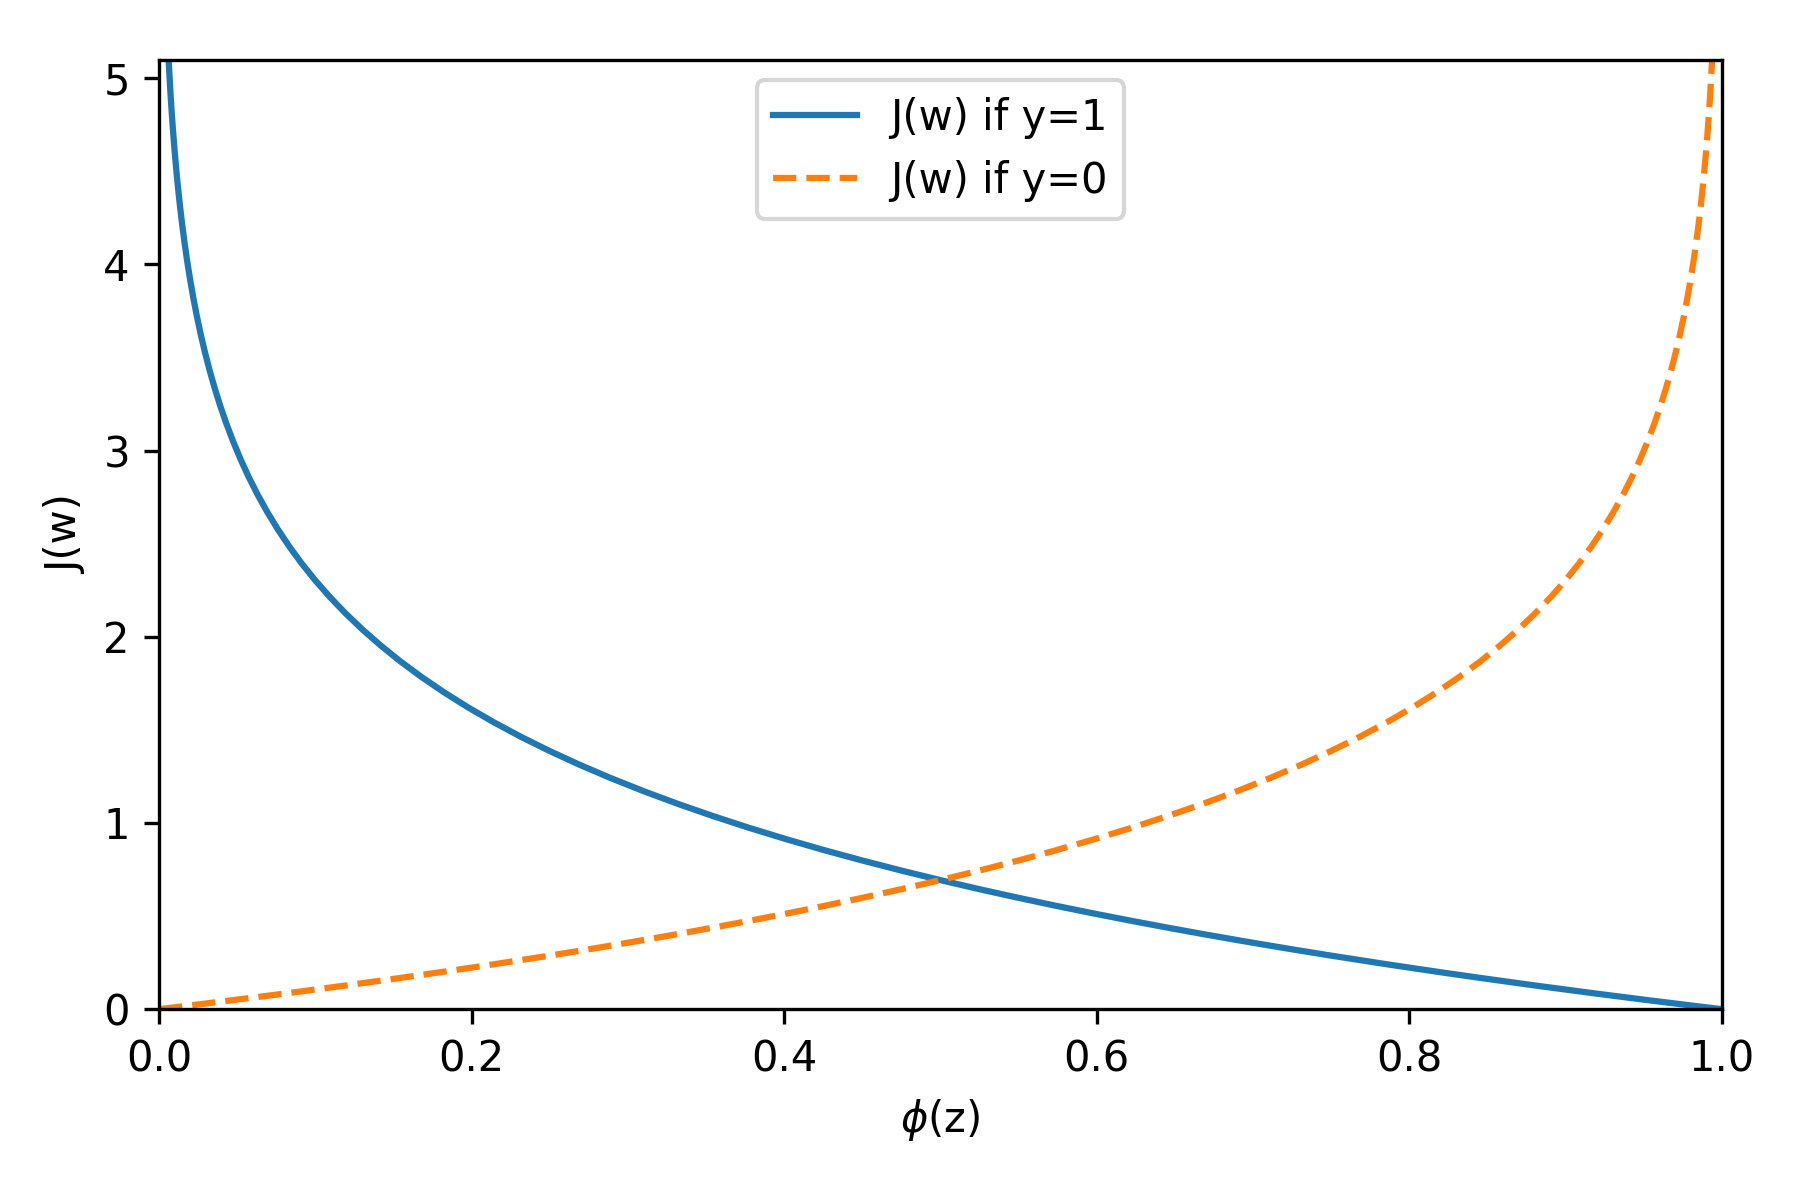
\includegraphics[width=9cm]{images/minimum_log_curve.png}
		\caption{Graphique d'une courbe de régression logistique ajustée aux données $(x_n , y_n)$. \cite[image de]{ml2008python}
		}
		\label{fig:minimum_log_curve}
	\end{figure}
	
	
	
	
	\section{Descente de gradient stochastique}
	Cette section est inspirée des articles écrites par Léon Bottou et al, dans  \cite{bottou2012stochastic} 
	\cite{bottou2010large}
	\cite{framling2004scaled}
	\cite{bottou2018optimization}
	\cite{netrapalli2019stochastic}
	\cite{wijnhoven2010fast}.
	
	\subsection{Descente de gradient (Gradient Descent)}
	
	
	Il a souvent été proposé de minimiser le risque empirique [E] en utilisant la descente de gradient (GD). Chaque itération met à jour les poids w en fonction du gradient de [E] \cite{bottou2012stochastic}.\\
	
	\lipsum[1] \\ 
	
	$$A = \begin{pmatrix}
		x_{11} & x_{12} & x_{13} & \cdots & x_{1n} \\
		x_{21} & x_{22} & x_{23} & \cdots & x_{2n} \\
		\vdots & \vdots & \vdots & \ddots & \vdots \\
		x_{m1} & x_{m2} & x_{m3} & \cdots & x_{mn} 
	\end{pmatrix}$$
	
	
	\lipsum[4]
	\subsubsection{Pourquoi stochastique?}
	Descente de gradient stochastique (SGD) 
	
	L'algorithme de descente de gradient stochastique (SGD) est une simplification drastique. Au lieu de calculer exactement le gradient de E n (f w ), chaque itération estime ce gradient sur la base d'un seul exemple z t pris au hasard \cite{bottou2012stochastic} :
	$$
	{\displaystyle w:=w-\eta \nabla Q(w)=w-{\frac {\eta }{n}}\sum _{i=1}^{n}\nabla Q_{i}(w),}
	$$
	\lipsum[1]	
	\subsection{La convergence de la descente de gradient stochastique}
	\lipsum[1]	
	
	\section{Les optimiseurs SGD}
	\subsection{Perceptron Optimizer}
	
	Le perceptron est un modèle simplifié d'un neurone biologique . Alors que la complexité des modèles de neurones biologiques est souvent nécessaire pour bien comprendre le comportement neuronal, la recherche suggère qu'un modèle linéaire de type perceptron peut produire certains comportements observés dans de vrais neurones.
	
	Un perceptron est une unité de réseau neuronal (un neurone artificiel) qui effectue certains calculs pour détecter des caractéristiques ou une intelligence économique dans les données d'entrée.
	Et aussi en Machine Learnig (apprentissage automatique), le perceptron est un algorithme d'apprentissage supervisé de classificateurs binaires (qui se fait dans la régression logistique). 
	Un classificateur binaire est une fonction qui peut décider si une entrée, représentée par un vecteur de nombres, appartient ou non à une classe spécifique. \cite{freund1999large} Il s'agit d'un type de classificateur linéaire , c'est-à-dire un algorithme de classification qui fait ses prédictions sur la base d'une fonction prédictive linéaire combinant un ensemble de poids avec le vecteur de caractéristiques .
	
	Le premier concept de règle d'apprentissage du perceptron, a été publié par Frank Rosenblatt [??],  basé sur le modèle neuronal MCP(???). 
	
	(F. Rosenblatt, The Perceptron, a Perceiving and Recognizing Automaton. Cornell Aeronautical Laboratory, 1957).
	
	Avec sa règle de perceptron, Rosenblatt a proposé un algorithme qui apprendrait automatiquement les coefficients de poids optimaux qui sont ensuite multipliés par les caractéristiques d'entrée afin de décider si un neurone se déclenche ou non. Dans le cadre de l'apprentissage supervisé et de la classification, un tel algorithme pourrait alors être utilisé pour prédire si un échantillon appartient à une classe ou à l'autre [Python machine learning].
	
	Il est important de noter que la convergence du perceptron n'est garantie que si les deux classes sont linéairement séparables et que le taux d'apprentissage est suffisamment faible. Si les deux classes ne peuvent pas être séparées par une limite de décision linéaire, nous pouvons définir un nombre maximum de passages sur l'ensemble de données d'apprentissage (époques) et/ou un seuil pour le nombre d'erreurs de classification tolérées - le perceptron n'arrêterait jamais de mettre à jour les poids autrement:
	
	\subsection{Neurone linéaire adaptatif (ADALINE)}
	\lipsum[1]




%#######################################################################################
%
%	PART III
%
%#######################################################################################

%\ctparttext{\centering L'entrainement d'un modèle de Machine Learning par la classification avec un dataset de images. La mise en place, l'implémentation de notre modèle entrainé dans une application desktop pour \\???.       } 

%\textcolor{teal}{\part{Implémentation \& Expérimentation }}

%\textcolor{teal}{\part{Expérimentation }}

%#

%#############################################################################
%
%              						CHAPTER 
%
%#############################################################################

\textcolor{cyan}{\chapter{Expérimentation}}

\section{Implémentation des optimiseurs pour l'ANPR}

	\subsection{Matériel utilisé pour l'implementation}
	\lipsum[1].
	\subsection{Élaboration de la base de données {Dataset}}
	
	\lipsum[1]
	
	\subsection{Construction d'un modèle d'entrainment}
	\subsection{Former le modèle}
	\lipsum[1]
	
	\subsubsection{Évaluer l'efficacité du modèle}
	%\cite{deepa2021ai,ahadjitse2013reconnaissance}\cite{amari1993backpropagation}. 
	
	\lipsum[1]
	

\section{Expérimentation de résultat}
	\subsection{Analyse des données } 
	\lipsum[1] 
	\subsection{Les jeux des testes}
	\lipsum[1] 
	
	\subsection{Critères d'évaluation des tests}
	\lipsum[1] 
	\subsubsection{Matrice de confusion}
	\lipsum[1] 
	\subsection{Résultats d'expérimentation}
	\subsubsection{Utiliser le modèle formé pour faire des prédictions}
	\lipsum[1] 
	\subsubsection{Problèmes posés}
	\lipsum[1] 
	\subsection{Sommaire du chapitre}
	\lipsum[1] 
	\lipsum[1] 
	\lipsum[1] 
	




%=======================================================================================
%#
%

\addcontentsline{toc}{chapter}{Conclusion}

\textcolor{cyan}{\chapter*{Conclusion générale}}
	\lipsum[2]
	%\cite{framling2004scaled} \cite{friess1999kernel}.
	\lipsum[3]
	\lipsum[1]
	
	





%#######################################################################################
%
%	THESIS CONTENT - APPENDICES 
%
%#######################################################################################


\appendix

%\ctparttext{Quelques programmes }

\part*{Annexes et Bibliographies} % New part of the thesis for the appendix

%


%\addcontentsline{toc}{chapter}{Annexe A : Adaline SGD Training Code}
\chapter{Adaline SGD Training Code}
%\addcontentsline{toc}{chapter}{Annexe B : Result of Test}
\chapter{Result of Test}
%\addcontentsline{toc}{chapter}{Annexe C : Dataset \& Model}
\chapter{Dataset \& Model}
	\lipsum[1]. \cite{ahadjitse2013reconnaissance} \\
	\lipsum[3]
	\cite{deepa2021ai}.
	\cite{bottou2012stochastic}.
	\cite{framling2004scaled}\\
	
	Lorem ipsum dolor sit amet, consectetur adipiscing elit, sed do eiusmod tempor incididunt ut labore et dolore magna aliqua. (\eg, \cite{lydia2019adagrad} \cite{netrapalli2019stochastic} \cite{caruana2006empirical}.)

%\cite[][page 176-195]{bishop2006pattern}




%% Appendix A

\chapter{Appendix Test}

%----------------------------------------------------------------------------------------

\lipsum[13-14]

%----------------------------------------------------------------------------------------

\section{Appendix Section Test}
\lipsum[15]

\graffito{More dummy text}
\lipsum[16]

%----------------------------------------------------------------------------------------

\section{Another Appendix Section Test}
\lipsum[17]

\begin{table}
\myfloatalign
\begin{tabularx}{\textwidth}{Xll} \toprule
\tableheadline{labitur bonorum pri no} & \tableheadline{que vista}
& \tableheadline{human} \\ \midrule
fastidii ea ius & germano &  demonstratea \\
suscipit instructior & titulo & personas \\
\midrule
quaestio philosophia & facto & demonstrated \\
\bottomrule
\end{tabularx}
\caption[Autem usu id]{Autem usu id.}
\label{tab:moreexample}
\end{table}

\lipsum[18]

There is also a useless Pascal listing below: \autoref{lst:useless}.

\begin{lstlisting}[float=b,language=Pascal,frame=tb,caption={A floating example (\texttt{listings} manual)},label=lst:useless]
for i:=maxint downto 0 do
begin
{ do nothing }
end;
\end{lstlisting} % Appendix A
%% Appendix X

\chapter{Appendix Title}

%----------------------------------------------------------------------------------------

% Content begins here % Appendix B - empty template

%----------------------------------------------------------------------------------------
%	POST-CONTENT THESIS PAGES
%----------------------------------------------------------------------------------------
%\bibliographystyle{plain}
%\addcontentsline{toc}{chapter}{\tocEntry{\bibname}}
%\bibliography{Bibliography}
%\cleardoublepage% Bibliography

\label{app:bibliography} % Reference the bibliography elsewhere with \autoref{app:bibliography}

\manualmark % Work-around to have small caps also here in the headline
\markboth{\spacedlowsmallcaps{\bibname}}{\spacedlowsmallcaps{\bibname}} % Work-around to have small caps also
%\phantomsection
\refstepcounter{dummy}

\addtocontents{toc}{\protect\vspace{\beforebibskip}} % Place the bibliography slightly below the rest of the document content in the table of contents
\addcontentsline{toc}{chapter}{\tocEntry{\bibname}}

\printbibliography

 % Bibliography

%========================================================================================
%========================================================================================

\label{app:bibliography} % Reference the bibliography elsewhere with \autoref{app:bibliography}

\manualmark % Work-around to have small caps also here in the headline
\markboth{\spacedlowsmallcaps{\bibname}}{\spacedlowsmallcaps{\bibname}} % Work-around to have small caps also
%\phantomsection
\refstepcounter{dummy}

\addtocontents{toc}{\protect\vspace{\beforebibskip}} % Place the bibliography slightly below the rest of the document content in the table of contents
\addcontentsline{toc}{chapter}{\tocEntry{\bibname}}

\printbibliography



%\cleardoublepage% Declaration

\refstepcounter{dummy}
\pdfbookmark[0]{Declaration}{declaration} % Bookmark name visible in a PDF viewer

\chapter*{Declaration} % Declaration section text

\thispagestyle{empty}
 

Ce rapport de stage effectué à Kamoto Copper Company a été rédigé par\\ \textbf{TSHELEKA KAJILA Hassan}, étudiant de l'\textsc{Université Nouveaux Horizons}, conformément aux exigences du diplôme de Licencié en Sciences informatique, département : \textbf{Calcul Scientifique}

\bigskip
 
\noindent\textit{\myLocation, \myTime}

\smallskip

\begin{flushright}
\begin{tabular}{m{5cm}}
\\ \hline
\centering\myName \\
\end{tabular}
\end{flushright}
 % Declaration

%\cleardoublepage% Colophon (a brief description of publication or production notes relevant to the edition)

\pagestyle{empty}

\hfill

\vfill

\pdfbookmark[0]{Colophon}{colophon}

\section*{Colophon}
Cette étude a été très enrichissant pour moi, car il m'a permis de découvrir le domaine du Machine Learning, apprentissage supervisé, ses acteurs. Elle m'a permis de participer concrètement à ses enjeux au travers mes missions en apprentissage supervisé et la vision par ordinateur. Je préfère ainsi m'orienter vers un domaine lié à ma mission en Calcul Scientifique et le Data Science.



%This document was typeset using the typographical look-and-feel \texttt{classicthesis} developed by Andr\'e Miede. The style was inspired by Robert Bringhurst's seminal book on typography ``\emph{The Elements of Typographic Style}''. \texttt{classicthesis} is available for both \LaTeX\ and \mLyX: 

\begin{center}
\url{https://www.katangamining.com}
\end{center}
{Ce mémoire pour le travail de fin de cycle \textsf{$2021-2021$} qui traite la thématique du \texttt{Machine Learning \& Computer Vision} a été rédigé par {TSHELEKA KAJILA Hassan}, étudiant de l'\textsc{Université Nouveaux Horizons}, conformément aux exigences du diplôme de Licencié en Sciences informatique, département : \emph{Calcul Scientifique}.}


\begin{center}
\url{https://www.unhorizons.org}
\end{center}
 
\bigskip

\noindent\finalVersionString % Colophon

%----------------------------------------------------------------------------------------

\end{document}
